%
%  THESISBOEK
%
%  Dit bestand zorgt voor algemene (layout)definities, en groepeert de
%  afzonderlijke LaTeX-files tot een geheel.
%
%  @author Erwin Six, David De Reu, Brecht Vermeulen
%

\documentclass[11pt,a4paper,oneside,notitlepage]{book}
\usepackage[english,dutch]{babel}

\usepackage{mathtools}
\usepackage{verbatim}
% marges aanpassen
% (opmerking: moet *voor* inclusie van fancyhdr package komen)
\setlength{\hoffset}{-1in}
\setlength{\voffset}{-1in}
\setlength{\topmargin}{2cm}
\setlength{\headheight}{0.5cm}
\setlength{\headsep}{1cm}
\setlength{\oddsidemargin}{3.5cm}
\setlength{\evensidemargin}{3.5cm}
\setlength{\textwidth}{16cm}
\setlength{\textheight}{23.3cm}
\setlength{\footskip}{1.5cm}

\usepackage{fancyhdr}
\usepackage{graphicx}
% \usepackage[colorlinks]{hyperref}

\pagestyle{fancy}

\renewcommand{\chaptermark}[1]{\markright{\MakeUppercase{#1}}}
\renewcommand{\sectionmark}[1]{\markright{\thesection~#1}}

\newcommand{\headerfmt}[1]{\textsl{\textsf{#1}}}
\newcommand{\headerfmtpage}[1]{\textsf{#1}}

\fancyhf{}
\fancyhead[LE,RO]{\headerfmtpage{\thepage}}
\fancyhead[LO]{\headerfmt{\rightmark}}
\fancyhead[RE]{\headerfmt{\leftmark}}
\renewcommand{\headrulewidth}{0.5pt}
\renewcommand{\footrulewidth}{0pt}

\fancypagestyle{plain}{ % eerste bladzijde van een hoofdstuk
  \fancyhf{}
  \fancyhead[LE,RO]{\headerfmtpage{\thepage}}
  \fancyhead[LO]{\headerfmt{\rightmark}}
  \fancyhead[RE]{\headerfmt{\leftmark}}
  \renewcommand{\headrulewidth}{0.5pt}
  \renewcommand{\footrulewidth}{0pt}
}

% anderhalve interlinie (opm: titelblad gaat uit van 1.5)
\renewcommand{\baselinestretch}{1.5}

% indien LaTeX niet goed splitst, neem je woord hierin op, of evt om splitsen 
% te voorkomen
\hyphenation{ditmagnooitgesplitstworden dit-woord-splitst-hier}

\begin{document}

% titelblad (voor kaft)
%  Titelblad

% Opmerking: gaat uit van een \baselinestretch waarde van 1.5 (die moet
% ingesteld worden voor het begin van de document environment)

\begin{titlepage}

\setlength{\hoffset}{-1in}
\setlength{\voffset}{-1in}
\setlength{\topmargin}{1.5cm}
\setlength{\headheight}{0.5cm}
\setlength{\headsep}{1cm}
\setlength{\oddsidemargin}{3cm}
\setlength{\evensidemargin}{3cm}
\setlength{\footskip}{1.5cm}
\enlargethispage{1cm}
% \textwidth en \textheight hier aanpassen blijkt niet te werken

\fontsize{12pt}{14pt}
\selectfont

\begin{center}


\includegraphics[height=2cm]{fig/ruglogo}

\vspace{0.5cm}

Faculteit Ingenieurswetenschappen en Architectuur\\
%Vakgroep Informatietechnologie\\
%Voorzitter: Prof.~Dr.~Ir.~P.~LAGASSE

\vspace{3.5cm}

\fontseries{bx}
\fontsize{17.28pt}{21pt}
\selectfont
Een privacyvriendelijk aanbevelingssysteem\\
voor mobiele toestellen
\fontseries{m}
\fontsize{12pt}{14pt}
\selectfont

\vspace{.6cm}

door 

\vspace{.4cm}

Thorwald Frederik Lambrecht

\vspace{3.5cm}

Interne promotor: Marleen Denert\\
Externe promotor: Luc Martens
\\Externe begeleider: Toon De Pessemier
%Promotor: Prof.~Dr.~Ir.~P.~DEMEESTER\\
%Scriptiebegeleider: Ir.~B.~VERMEULEN\\

\vspace{2cm}

Scriptie ingediend tot het behalen van de academische graad van\\
Master of Science in de industri\"ele wetenschappen: informatica

\vspace{1cm}

Academiejaar 2014--2015

\end{center}
\end{titlepage}


% lege pagina (!!)

% titelblad (!!)

% geen paginanummering tot we aan de inhoudsopgave komen
\pagestyle{empty}

% voorwoord met dankwoord en toelating tot bruikleen (ondertekend)
%  Voorwoord (dankwoord) en toelating tot bruikleen

\newpage

\noindent \textbf{\huge Voorwoord}

\vspace{1.5cm}

\noindent


Graag wou ik de volgende personen bedanken voor hun hulp bij het tot stand komen van deze masterscriptie. Mijn begeleiders tijdens deze masterproef: mevrouw Marleen Denert voor de uitgebreide feedback; en meneer Toon De Pessemier, voor het altijd paraat staan bij vragen of problemen.
Verder een dankwoord voor mijn vrienden in het bijzonder Jeroen De Ridder en Laetitia Van Espen voor de morele steun en hulp bij het testen van het project.

\addvspace{4cm}

\noindent Thorwald Frederik Lambrecht, januari 2015\newpage

\noindent \textbf{\huge Toelating tot bruikleen}

\vspace{1.5cm}

\noindent
``De auteur geeft de toelating deze scriptie voor consultatie beschikbaar
te stellen en delen van de scriptie te kopi\"eren voor persoonlijk
gebruik.\\
Elk ander gebruik valt onder de beperkingen van het auteursrecht,
in het bijzonder met betrekking tot de verplichting de bron uitdrukkelijk
te vermelden bij het aanhalen van resultaten uit deze scriptie.''

\addvspace{4cm}

\noindent Thorwald Frederik Lambrecht, januari 2015


% overzicht
%%  Overzichtsbladzijde met samenvatting

\newpage

{
\setlength{\baselineskip}{14pt}
\setlength{\parindent}{0pt}
\setlength{\parskip}{8pt}

\begin{center}

\noindent \textbf{\huge
Ontwerp van een performante\\[8pt]
gedistribueerde CORBA--monitor
}

door 

David DE REU

Scriptie ingediend tot het behalen van de academische graad van\\
burgerlijk ingenieur in de computerwetenschappen

Academiejaar 2001--2002

Promotor: Prof.~Dr.~Ir.~P.~DEMEESTER\\
Scriptiebegeleider: Ir.~B.~VERMEULEN

Faculteit Toegepaste Wetenschappen\\
Universiteit Gent

Vakgroep Informatietechnologie\\
Voorzitter: Prof.~Dr.~Ir.~P.~LAGASSE

\end{center}

\section*{Samenvatting}

% TODO: samenvatting

Hier komt de samenvatting.


\section*{Trefwoorden}

% TODO: trefwoorden

Hier komen trefwoorden.

}

\newpage % strikt noodzakelijk om een header op deze blz. te vermijden


\pagestyle{fancy}
\frontmatter

% inhoudstafel
\tableofcontents

% opmaak voor het eigenlijke boek; onderstaande lijnen
% weglaten als de eerste regel van een nieuwe alinea moet
% inspringen in plaats van extra tussenruimte
%\setlength{\parindent}{0pt}
%\setlength{\parskip}{0.5\baselineskip plus 0.5ex minus 0.2ex}
%\setlength{\parskip}{1ex plus 0.5ex minus 0.2ex}

% hoofdstukken
\mainmatter

% hier worden de hoofdstukken ingevoegd (\includes)
\chapter{Inleiding}
Een aanbevelingssysteem is een handig middel om zich een weg te banen doorheen de enorme hoeveelheid content die sommige webapplicaties aanbieden. Het laat ons toe snel interessante en persoonsgerichte items te vinden.
Aanbevelingssystemen kunnen mensen nieuwe vrienden leren kennen of zorgen voor een boost in verkoopcijfers door gerichte marketing. Ze kunnen ook gebruikt worden om de gebruiker nieuwe dingen aan te leren. Zo zal bijvoorbeeld OWL \cite{Linton00owl} gebruikers nieuwe shortcuts aanreiken voor veelgebruikte commando's in een bepaald programma. Het kan ook een doel zijn om een community van gebruikers te cre\"eren rond items. Een voorbeeld hiervan is Tripadvisor.com, waar men niet beoogt om zoveel mogelijk reservaties te verkrijgen maar eerder een community uit te bouwen die elkaar helpt bij het kiezen tussen hotels. 
Service providers die klassieke aanbevelingssystemen gebruiken houden vaak veel persoonlijke data bij op hun servers. De data van een persoon wordt bijgehouden in zijn gebruikersprofiel. Google heeft al aangegeven dat het alle data van \'e\'en persoon van zijn verschillende services bijhoudt in \'e\'en profiel. 

Het bijhouden van deze gigantische hoeveelheden data brengt vragen met zich mee:
\begin{itemize}
 
\item Wordt deze data wel correct beheerd? 
\item Welke risico's zijn er voor onze privacy?
\item Kan misbruik vermeden worden met alternatieve privacyvriendelijkere methodes?
\end{itemize}

Aanbevelingen zijn logischerwijs gezien beter of nauwkeuriger naarmate het systeem beschikt over meer gedetailleerde data. Er is dus in zekere zin een inherente wisselwerking tussen de privacy van de gebruiker en de nauwkeurigheid van het systeem. In deze masterproef concentreren we ons op hoe we de verschillende klassieke algoritmes om aanbevelingen te berekenen kunnen aanpassen zodat er minder risico is op privacy-inbreuken in verband met persoonlijke voorkeuren of persoonlijke informatie in het algemeen. Jammer genoeg hebben de mogelijkheden die al beschreven zijn in de literatuur een negatieve impact op de performantie van het algoritme en/of de nauwkeurigheid van de aanbevelingen. 
\begin{figure}[htpb]   
    \label{Figuur::wisselwerking}      
  \begin{center}    
 
\includegraphics[width=\textwidth,height=\textheight,keepaspectratio]{fig/wisselwerking}    
  \end{center}     
   \end{figure}\\
Het doel van deze masterproef is een optimale oplossing te vinden voor deze drievoudige wisselwerking en dus het algoritme te vinden dat enerzijds privacyvriendelijk is maar waarvan anderzijds de performantie aanvaardbaar is en de aanbevelingen goed en persoonlijk gericht zijn. Ook wordt er rekening gehouden met de mobiele setting: het algoritme moet bruikbaar zijn op een smartphone en dus rekening houden met beperkingen zoals rekenkracht en batterijgebruik.\\

Hiervoor bekijken we in hoofdstuk \ref{privacyklassiek} in paragraaf \ref{sec:klassiek} de klassieke aanbevelingssystemen en welke privacygevoelige data deze bijhouden. Vervolgens beschouwen we in paragrafen \ref{sec:privacy} tot en met \ref{sec:risicos} de betekenis van privacy in de context van een aanbevelingssysteem en de risico's die voorkomen bij bestaande aanbevelingssystemen. In hoofdstuk \ref{onderzoek} worden de bestaande oplossingen bestudeerd en geanalyseerd en bekeken welke het best scoort op de drie hoofdpunten, rekening houdend met een mobiele setting. De beste optie wordt als vertrekpunt genomen voor de uitwerking van een werkend privacyvriendelijk aanbevelingssysteem in hoofdstuk \ref{privacy_opl}. We kozen aan de client-kant voor een Androidapplicatie en aan de kant van de server kozen we voor Java.
 

\chapter{Privacyrisico's bij klassieke aanbevelingsystemen}
\label{privacyklassiek}

\section{Klassieke aanbevelingssystemen}
\label{sec:klassiek}
De verschillende soorten aanbevelingssystemen worden besproken, elke soort krijgt een korte uitleg waarin de werking ervan aan bod komt. Voor meer informatie omtrent de precieze werking wordt doorverwezen naar de vakliteratuur. \\Er wordt een onderscheid gemaakt tussen de volgende types.
\subsection{Niet-gepersonaliseerde statistieken}
Dit is de meest eenvoudige vorm van een aanbevelingssysteem. Bij deze statistieken wordt dus geen rekening gehouden met de beoordelingen of persoonlijke smaak van de gebruiker voor wie de aanbevelingen bedoeld zijn. Dit zijn statistieken zoals het gemiddelde aantal sterren beoordeeld door de hele community of items met het grootste aantal "vind-ik-leuk"'s. Andere statistieken die populair zijn, zijn productassociaties in de vorm van “mensen die x leuk vonden, vonden ook y leuk”. Externe community-data, zoals bijvoorbeeld meest verkochte items, wordt ook gebruikt.  Hoewel de niet-gepersonaliseerde statistieken duidelijk hun beperkingen hebben, zijn ze effici\"ent en kunnen ze erg nuttig zijn. 
\subsection{Content-based recommenders}
Het basisidee van inhoud-gebaseerde aanbevelingssystemen is om items te modelleren als vector in een meerdimensionale ruimte. Deze ruimte heeft als dimensies de relevante attributen van de items. De smaak van de gebruiker wordt ook voorgesteld als vector in deze ruimte, de \textit{uservector}. De uservector wordt opgesteld door zijn ratings van items die bepaalde attributen hebben. De interessante items worden meestal gevonden door die items te nemen waarvan de hoek tussen de itemvector en de uservector klein is. 
\subsection{Kennis-gebaseerde recommenders}
De gebruiker die aanbevelingen vraagt zal zijn voorkeuren aan het systeem geven. De gebruiker kan op de aangeboden items feedback geven zodat het systeem zijn aanbevelingen kan aanpassen.
\subsection{Collaborative Filtering recommenders}
\subsubsection{User-User Collaborative recommenders}
Bij user-user collaborative recommenders wordt de smaak van gebruikers vergeleken op basis van hun gegeven ratings met een  correlatieco\"effici\"ent zoals deze van Pearson. Als een gebruiker aanbevelingen vraagt, worden de gebruikers met een gelijkaardige smaak bepaald. De score voor een item wordt berekend door het gewogen gemiddelde te nemen van de scores voor dat item van de gebruikers met gelijkaardige smaak.
\subsubsection{Item-Item Collaborative recommenders}
Om een score voor een item te vinden voor een gebruiker wordt eerst gekeken naar de items waar hij wel een rating voor heeft. Indien het gezochte item volgens andere gebruikers gelijkaardig is (een gelijkaardige score heeft voor hen) aan wel beoordeelde items, neemt men het gewogen gemiddelde van de ratings van deze items.
\subsection{Andere aanbevelingssystemen}
\subsubsection{Demografic recommenders}
Als een persoonlijke voorkeur niet gekend is wordt afgegaan op kenmerken als leeftijd, geslacht en land van herkomst om aanbevelingen te genereren op basis van een stereotype.
\subsubsection{Social recommenders}
Deze aanbevelingssystemen maken gebruik van de vriendschapsbanden van een sociaal netwerk omdat aangenomen wordt dat vrienden gelijkaardige interesses hebben.
\subsubsection{Hybrid recommenders}
Zoals de naam aangeeft worden hier verschillende aanbevelingssystemen samen gecombineerd. Dit heeft als doel betere aanbevelingen te maken en de nadelen van de onderliggende systemen weg te werken.

\subsection{Singular Value Decomposition}
Singular Value Decomposition of singulierewaardenontbinding is een wiskundige techniek die toelaat aanbevelingen bij  collaborative filtering sneller te berekenen. De wiskundige basis ligt in de mogelijkheid een $m \times n$ matrix A op te splitsen in een product van drie matrices, respectievelijk een $m \times r$ matrix U, een $r \times r$ matrix $\sum$ met de singuliere waarden op de diagonaal en een $n \times r$ matrix V. 

\begin{figure}[htpb]   
    \label{Figuur::svd}      
  \begin{center}    
 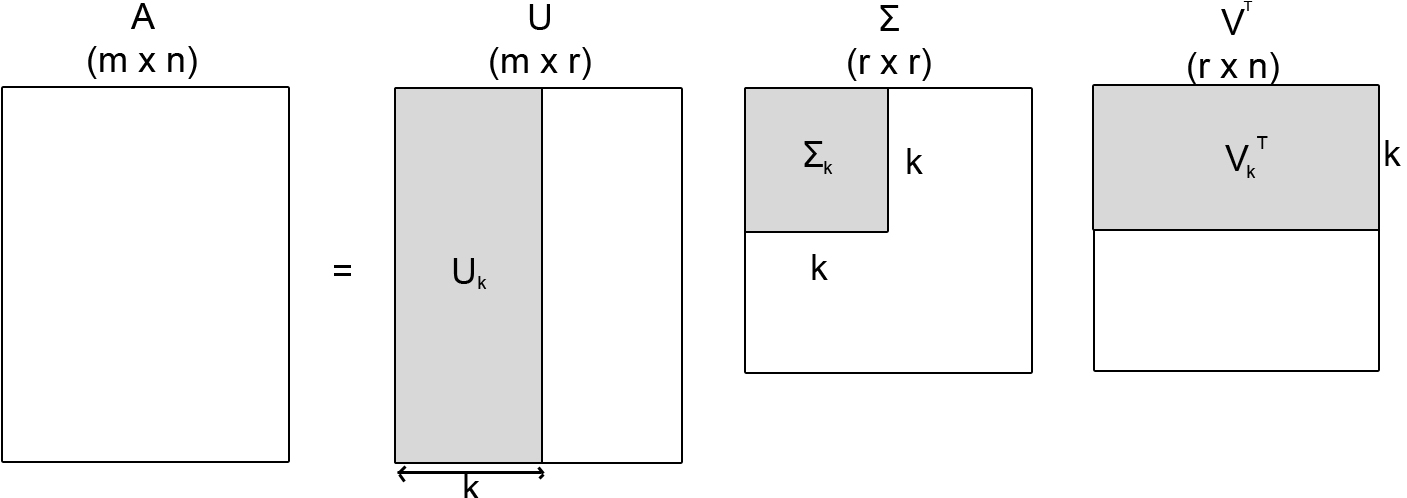
\includegraphics[scale=0.3]{fig/svd}    
  \end{center}   
    
   \end{figure}

 De singuliere waarden op de diagonaal van $\sum$ geven de belangrijkheid van deze bepaalde dimensie aan. Een deel van deze waarden is dicht bij 0 en dus kunnen deze  dimensies verwaarloosd worden en de matrix verkleind worden naar k rijen en kolommen. De scores in de U en de V matrix op deze verwaarloosde dimensies kunnen ook weggelaten worden. 
Deze techniek kan uitgevoerd worden op een traditionele userratingmatrix. Zonder SVD worden smaken van gebruikers vastgelegd als scores op bepaalde trefwoorden, zoals bij films bijvoorbeeld 5 \% comedie. Met SVD wordt de smaak van een gebruiker uitgedrukt in een kleiner aantal dimensies die een combinatie zijn van verschillende trefwoorden zonder verlies van veel informatie. Dit zorgt ervoor dat de data compacter kan worden bijgehouden en het algoritme minder computationeel werk heeft. Hierbij worden U de user-feature matrix en V de item-feature matrix genoemd.


\section{Evaluatie aanbevelingssystemen}
Een veelgebruikte basismetriek is Mean Absolute Error (MAE) of de gemiddelde absolute fout. Een rating voor een item wordt onzichtbaar gemaakt voor het systeem, waarna het systeem aangeeft welke score het zou geven op basis van alle andere bekende ratings. Het verschil tussen de vermomde score en de geraadde score is dus de fout. We berekenen het gemiddelde van de fouten voor elke rating en zo bekomen we het MAE. Een vergelijkbaar alternatief is de Mean Squared Error (MSE), die door kwadratering de grote fouten meer afstraft. De Root Mean Squared Error (RMSE) is hiervan de vierkantswortel zodat er een waarde bekomen wordt in de meer intu\"itieve originele schaal.
\begin{equation}
MAE = \frac{\sum_{ratings} (prediction - rating)}{\#ratings}
\end{equation}
\begin{equation}MSE = \frac{\sum_{ratings} (prediction - rating)^2}{\#ratings}
\end{equation}
\begin{equation}
RMSE = \sqrt{MSE}
\end{equation}
\textit{Precision} en \emph{recall} zijn ook veelgebruikte metrieken bij \emph{Information Retrieval} technieken. Ze focussen in tegenstelling tot de vorige metrieken niet op de nauwkeurigheid van een voorspellingswaarde. Precision en recall tonen respectievelijk hoeveel van de aanbevolen termen relevant zijn en het percentage van relevante items dat effectief wordt aanbevolen.




\section{Betrouwbaarheid}
De betrouwbaarheid van een aanbevelingssysteem leunt dicht aan bij de privacy. Hier kunnen we de volgende vragen stellen : 

\begin{itemize}
 
\item Is het systeem voldoende beschermd tegen aanvallen van buitenaf?
\end{itemize}
 Het aanbevelingssysteem moet allereerst bestand zijn tegen aanvallen van hackers die private informatie willen bemachtigen. In het verleden is er sprake geweest van buitenstaanders die ratings manipuleerden en extra gebruikersprofielen aanmaakten om extra informatie in te winnen over het gedrag van anderen. Een voorbeeld hiervan is een vroege aanval die de correlatieco\"efficient van Pearson misbruikte. De aanval maakte gebruik van het feit dat de co\"efficient \'e\'en is als twee gebruikers identiek dezelfde ratings hebben. Er werd met behulp van een beetje informatie over de gebruiker een valse account aangemaakt waarmee de co\"efficient \'e\'en werd, zo kon informatie achterhaald worden van de gebruiker. Deze aanvallen kunnnen bemoeilijkt worden door een minder transparant algoritme te gebruiken dat bijvoorbeeld gebruik maakt van Singular Value Decomposition. \\Daarbuiten moet het systeem ook voorkomen dat kwaadwillige gebruikers meerdere accounts aanmaken met als doel bepaalde items te promoten of in de vergetelheid te doen belanden. 
 
 \begin{itemize}
\item Beveelt het systeem de beste items wel aan?
\end{itemize}
 
  Het kan dat een service provider enkel deze items aanbeveelt die in stock zijn of waar het systeem het meest geld op verdient en niet deze die het interessantst zijn voor de gebruiker. 
  
 
\section{Privacy}
\label{sec:privacy}
Zoals eerder gezegd bestaat er een wisselwerking tussen privacy en accuraatheid van de aanbevelingen. Hier gaan we even in op wat men precies bedoelt met privacy. Privacy op het internet betekent privacy van informatie. In de literatuur verwijst men vaak naar de definitie van het Information Infrastructure Task Force (IITF).

 \begin{quotation}
"Privacy van informatie is het recht van een individu om controle uit te oefenen op de voorwaarden waaronder zijn persoonlijke informatie verzameld, gebruikt of bekendgemaakt wordt." \\-- Information Infrastructure Task Force \cite{pirs}
 \end{quotation}
Informatie wordt door een individu altijd gedeeld binnen een bepaalde \textit{scope}. Een scope wordt afgebakend door de grootte van het publiek, de manier waarop de informatie gebruikt mag worden en hoe lang dit mag.  Privacy betekent in deze context dus de informatie in dezelfde scope te houden als vooropgesteld door de persoon die informatie verstrekte \cite{pirs}.\\
Privacy van aanbevelingssystemen kan worden opgedeeld in twee soorten. Er is \textit{user-user privacy}, met betrekking tot de privacy tussen gebruikers onderling. Bij user-user privacy gaat het om wat een gebruiker online allemaal kan te weten komen over het gedrag van andere gebruikers. Sommige websites tonen de ratings en persoonlijke voorkeuren publiek maar bij andere sites is de vooropgestelde scope veel kleiner en deze houden persoonlijke voorkeuren priv\'e of onder vrienden.  

\begin{figure}[htpb]   
    \label{Figuur::usersystemprivacy}      
  \begin{center}    
 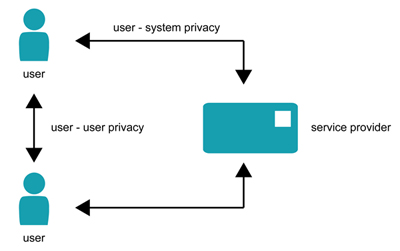
\includegraphics[scale=0.6,keepaspectratio]{fig/user-user-system-privacy}    
  \end{center}     
   \end{figure}
   
In tegenstelling tot sociale netwerken ligt bij aanbevelingssystemen het grootste probleem bij \textit{user-system privacy}. User-system privacy heeft betrekking tot de privacy kwesties tussen de gebruikers en de service provider. Een ander concept in privacy is \emph{deniability of preferences}, wat betekent dat je als gebruiker de mogelijkheid hebt om je eigen voorkeuren te ontkennen. Er is dus geen zekerheid voor een partij om de link te leggen tussen jou en je ratings.

\begin{figure}[htpb]   
    \label{Figuur::randomisatie}      
  \begin{center}    
 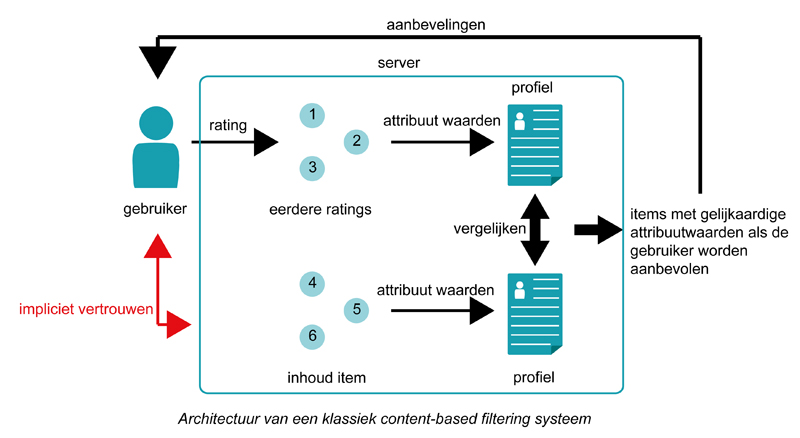
\includegraphics[scale=0.5]{fig/klassiek_systeem}    
  \end{center}   
   
   \end{figure}
Gebruikers hebben vaak een impliciet vertrouwen in de provider om verantwoord met hun data om te springen. 
\pagebreak
\section{Privacygevoelige data bij klassieke aanbevelingssystemen}
Veelgebruikte aanbevelingssystemen als content-based recommenders en collaborative filtering recommenders hebben toegang nodig tot persoonlijke voorkeuren om de berekeningen te kunnen doen. In de praktijk omvat dit expliciete data zoals commentaren, ratings, aankopen. Veel webapplicaties houden naast deze expliciete ook impliciete data bij zoals bezochte websites of bijvoorbeeld hoe lang een gebruiker naar een bepaald filmpje kijkt op Youtube. Ook knowledge-based recommenders verzamelen deze voorkeuren. Demografic recommenders hebben kennis nodig over de kenmerken van de gebruiker en social recommenders moeten natuurlijk weet hebben van het sociale netwerk.
\section{Privacyrisico's bij aanbevelingssystemen}
\label{sec:risicos}
\subsection{De gebruiker onderschat de omvang van de informatie die over hem wordt bijgehouden}
Van een smaakprofiel aan de hand van likes, het bijhouden van de operating systemversie met behulp van \emph{third-party} analytische tools tot het inkijken van de bezochte websites, een gebruiker is zich niet altijd bewust van de omvang van de data die van hem wordt bijgehouden\cite{pirs}. Dit is waarschijnlijk ook deels te wijten aan dat weinig gebruikers de privacyvoorwaarden lezen vooraleer een applicatie te starten. Uit een studie \cite{privdisc} bij 274 studenten bleek bijvoorbeeld 55.1\% de Facebook privacy policy niet gelezen te hebben. Hoofnagle et al. verrichte in \cite{hoofnagle} een studie over alle leeftijdsgroepen heen die hetzelfde vermoeden bevestigt. Hier blijkt  50\% van een groep van 975 personen nooit of bijna nooit de privacy policies op websites te lezen. Er is ook gewoonlijk weinig keuze, indien men de voorwaarden niet aanvaardt wordt de toegang tot de applicatie gewoonweg ontzegd. 
\subsection{Onterecht vertrouwen in de service provider}
\label{onterecht_vertrouwen}
\subsubsection{Het verkopen van data}
De informatie over de ratings en voorkeuren van gebruikers is erg interessant voor marketingdoeleinden. De verkoop van deze gegevens aan derde partijen ligt vaak niet in de lijn der verwachting van de gebruikers. Om de privacy te beschermen wordt deze data vaak geanonimiseerd. Toch biedt deze anonimisatie geen volledige bescherming. Zo hebben Narayanan en Schmatikov in \cite{Narayanan2008} de geanonimiseerde Netflix database kunnen deanonimiseren. Met een heel beperkte kennis van een gebruiker slaagden ze erin zijn records uit de databank te halen. Uit deze data konden ze politieke voorkeuren en andere gevoelige informatie afleiden.
\subsubsection{Data buiten de verwachte scope \cite{pirs}}
De gebruiker kan ervan uitgaan dat bepaalde informatie enkel zichtbaar is voor een beperkt publiek, terwijl dit in de praktijk niet het geval is, al dan niet moedwillig door de service provider. Er is bijvoorbeeld geen garantie voor gebruikers dat het personeel van het aanbevelingssysteem hun persoonlijke data niet doorneemt of niet voldoende beschermt.\\

Eens informatie van de gebruiker op het internet staat is ze helaas moeilijk te verwijderen. De service provider zelf vermoeilijkt dit soms aangezien er commerci\"ele waarde aan deze gegevens hangt. Het kan dus zijn dat data langer aanwezig is dan de gebruiker wil.


\section{Preventie van inbreuken op de privacy}
Nu er inzicht verkregen is welke risico's de gebruiker loopt kan er onderzocht worden wat er kan doen gebeuren inbreuken op zijn privacy te voorkomen.

\subsection{De gebruiker informeren}

Uit cijfers van Hoofnagle et al. \cite{hoofnagle} kan ook opgemaakt worden dat bij 55\% van de 975 ondervraagden de bezorgdheid rond online privacy de laatste vijf jaar is gestegen. Uit deze groep geeft 48\% aan dat de hoofdreden hiervoor is dat ze meer over de risico's ervan weten. De gebruiker informeren zou dus een positief effect kunnen hebben op zijn bezorgdheid en zijn privacy-eisen. Anderzijds gaf 77\% van de studenten in \cite{privdisc} aan dat de reden waarom de privacy policies niet gelezen werden was omdat de studenten het te veel moeite vonden of de policy moeilijk te begrijpen was. Dit toont aan dat initiatieven als "The Platform for Privacy Preferences (http://www.w3.org/P3P/)" nuttig zijn. Dit project zorgt voor een gestandaardiseerd formaat waarin websites en applicaties hun privacy policy kunnen defini\"eren. Dit formaat kan dan eenvoudig gelezen worden door een applicatie of plug-in aan de clientkant. Deze applicatie kan dan deze informatie op een gebruiksvriendelijke en begrijpbare manier tonen en eventueel op basis ervan indien de gebruiker dit wenst geautomatiseerde beslissingen nemen in zijn plaats. Zo hoeft de user de policies niet altijd te lezen. Alternatief kan de gebruiker ook bewuster gemaakt worden van de risico's die hij loopt door de privacy-informatie prominenter te tonen. Een studie van Tsai et Al. \cite{tsaitsai} toont aan dat users indien ze privacy-informatie prominent aanwezig zien meer geneigd zijn om van betrouwbaardere sites te kopen die duurder mogen zijn terwijl ze anders enkel keken naar de kleinste prijs. 

\subsection{Privacywetten}
De wetten omtrent de privacy vormt de middengrond tussen enerzijds de bescherming van de gebruiker en anderzijds de bedrijven die gerichte marketing willen voeren. Of het nu de Europese richtlijnen zijn als de Europese wetgeving rond databescherming en de Europese wetgeving rond de e-Privacy of het Amerikaanse Federal Trade Commission Act, beide lopen achter de technologie aan. Wetten worden ook vaak pas ingevoerd  nadat er iets fout is gelopen en niet om inbreuken te voorkomen.

\subsection{Privacyvriendelijke methodes}
Een alternatief is natuurlijk om met behulp van privacyvriendelijke algoritmes aanbevelingen te berekenen. Hier wordt op in gegaan de volgende hoofdstukken.



\chapter{Onderzoek Bestaande Privacyvriendelijke Methodes}
\label{onderzoek}

\section{Bruikbare Encryptiesystemen}

\subsection{Homomorfe encryptie}
Homomorfe encryptie is een encryptietechniek die toelaat om bewerkingen op cijferteksten uit te voeren die overeenkomen met bewerkingen op de onderliggende data van deze cijferteksten. Er wordt een onderscheid gemaakt tussen additief en multiplicatief homomorf. Additieve cryptosystemen bevatten een operatie op twee cijferteksten die overeenkomt met de som van de data. De volgende formules \cite{erkin:generating} tonen deze additieve homomorfe eigenschap bij additieve systemen op basis van vermenigvuldiging. De encryptie $\mathcal{E}$ en decryptie $\mathcal{D}$ van de berichten $m_1$ en $m_2$ gebeuren logischerwijs met de bij elkaar horende publieke en private sleutel.

\begin{equation}\label{pearson}\mathcal{D}(\mathcal{E}(m_1).\mathcal{E}(m_2)) = m1 + m2
\end{equation}
Als gevolg hiervan kan ook de vermenigvuldiging berekend worden van de data met een niet ge\"encrypteerd getal.

\begin{equation}\label{pearson}\mathcal{D}((\mathcal{E}(m))^a) = m.a
\end{equation}
De gebruikte systemen, Paillier en DGK, ondersteunen beide de additieve homomorfe eigenschap op basis van vermenigvuldiging.

Voor de volledigheid is dit de formule voor multiplicatieve homomorfe systemen op basis van vermenigvuldiging.

\begin{equation}\label{pearson}\mathcal{D}(\mathcal{E}(m_1).\mathcal{E}(m_2)) = m1 . m2
\end{equation}
\subsubsection{Een Pailliercryptosysteem}
\label{paillier}
De encryptie in een Pailliersysteem is op de volgende manier gedefinieerd \cite{erkin:generating}:

\begin{equation}\label{pearson}\mathcal{E}(m,r) = g^m.r^n mod n^2
\end{equation}

Hier is n het product van p en q, twee grote priemgetallen. De publieke sleutel wordt gevormd door (n,g) en de private sleutel door (p,q). Het gebruik van de randomwaarde r zorgt ervoor dat het Pailliersysteem semantisch veilig is. Dit betekent dat elke encryptie van dezelfde plaintext nooit resulteert in dezelfde ciphertext. Deze eigenschap komt later van pas in de privacyvriendelijke oplossing.
Zoals eerder vermeld ondersteunt het Pailliercryposysteem de additieve homomorfe eigenschap op basis van vermenigvuldiging. 
\begin{comment}
Deze eigenschap kan snel aangetoond worden. 
\end{comment}
\subsubsection{Een Damgard, Geisler en Kroigaard cryptosysteem (DGK)}
\label{dgk}
Het DGKsysteem ondersteunt net als Paillier de additieve homomorfe eigenschap op basis van vermenigvuldiging en is net als Paillier semantisch veilig. Voor hetzelfde veiligheidsniveau heeft het echter een kleinere berichtgrootte en het is dus effici\"enter dan Paillier. Het is vooral zeer effici\"ent in het nagaan met de private sleutel of een ge\"encrypteerde bit op nul staat.

\section{Bestaande Privacyvriendelijke Methodes}



\subsection{Op basis van anonimisatie}

\subsubsection{Agent-Based aanpak door Cissée en Albayrak \cite{CisseeAAP}}

Deze werkwijze spitst zich toe op een Information Filtering (IF) systeem.

Het IF systeem wordt opgesplitst in drie entiteiten: de user, de provider en de filter entiteit. De entiteiten worden in de praktijk door agents vertegenwoordigd. In tegenstelling tot sommige applicaties, waar de provider en de filter door dezelfde partij worden vertegenwoordigd, is dit bij deze werkwijze niet vereist. Dit zorgt voor een meer generieke oplossing. 

Het systeem houdt per entiteit rekening met het respectievelijk privacy aspect. Informatie die mogelijks gelinkt kan worden aan een gebruiker kan niet permanent opgevraagd worden door andere entiteiten. De enige informatie die de provider permanent prijsgeeft zijn de aanbevelingen zelf. Het filteralgoritme kan niet door externe bronnen geraadpleegd worden. Private data van de entiteiten (uitgezonderd de aanbevelingen) wordt enkel tijdelijk beschikbaar gemaakt voor een andere entiteit. Dit wordt mogelijk gemaakt doordat bepaalde entiteiten de communicatie van andere entiteiten kunnen controleren.

Het basisidee is dat de user en provider entiteiten hun data sturen naar de filter entiteit.  De gebruikersdata bestaat uit zijn ratings. De data van de provider bestaat uit een enorme hoeveelheid items, enkel relevante items worden naar de filter gestuurd. Deze filter entiteit berekent de aanbevelingen en verwijdert private data van beide entiteiten. De communicatie tussen de filter entiteit en de user en provider entiteiten gebeurt via een relay entiteit. Die zorgt ervoor dat de zoekopdrachten naar de provider anoniem gebeuren en dus niet gelinkt kunnen worden aan de filterentiteit die tijdelijk de persoonlijke data bevat.

In dit artikel kan de op agents gebaseerde aanpak enkel gebruikt worden voor content-based filtering of knowledge-based filtering. Om ook user-user collaborative filtering toe te laten kan  een match-maker module ge\"integreerd worden, beschreven in \cite{CisseeThesis2009}. Hier heeft de provider entiteit de extra taak om de gelijkenissen tussen gebruikers te bepalen. De privacy van de gebruiker wil men garanderen door met pseudoniemen te werken aan de kant van de provider en anonieme communicatie van de provider naar de user toe.\\\\
Belangrijke kenmerken : 
\begin{itemize}


\item Berekeningen van de aanbevelingen gebeuren in de vertrouwde filter entiteit.
\end{itemize}
Voordelen : 
\begin{itemize}


\item Houdt ook rekening met de privacy van de provider en het gebruikte algoritme.

\end{itemize}
Nadelen:
\begin{itemize}
\item Anonimisatie van de zoekopdrachten door middel van relay entiteiten bij het kennis-gebaseerde aanbevelingssysteem zou kunnen leiden tot re\"identificatie van de gebruikers. Dit kan ook het geval zijn bij het gebruik van pseudoniemen in het user-user collaborative filtering systeem.
\item De filter agent moet worden vertrouwd door de gebruiker en mag niet samenvallen met de provider.
\item Het aanmaken van agents en bijhorende communicatieplatformen cre\" eert extra overhead wat de performantie benadeelt. Een aanbeveling met dit systeem duurt ongeveer 10 maal zo lang als een normale aanbeveling.

\end{itemize}
\pagebreak
\subsection{Op basis van verstoring door randomisatie}
\label{randomisatie}
\subsubsection{Randomisatie aanpak op basis van Singular Value Decomposition door Polat en Du \cite{Polat:2005:SCF:1066677.1066860}}

Deze werkwijze focust enkel op de privacy van de gebruiker. De gebruiker zal zijn gegevens “vermommen” of eerder verstoren en deze verstoorde data naar de server sturen. De verstoring gebeurt op een manier zodat de server niet de correcte persoonlijke data van de user kent maar eerder de range kent waartussen de waarden liggen. Toch kan de server op deze waarden Collaborative Filtering alsnog uitvoeren. Dit is mogelijk omdat SVD gebaseerd is op geaggregeerde gegevens en niet op individuele waarden.

Men voegt de verstoring toe in drie stappen:
\begin{enumerate}
\item De server beslist welke verdeling men zal gebruiken om de data te verstoren en laat dit de gebruikers weten. Mogelijkheden zijn bijvoorbeeld een uniforme verdeling of een Gaussverdeling.
\item Elke gebruiker berekent Z-scores \footnote{De Z-score of gestandaardiseerde vorm van een stochastische variabele $X$ met verwachtingswaarde $\mu$ en standaardafwijking $\sigma$ is de afwijking van zijn verwachtingswaarde, uitgedrukt in eenheden van de standaardafwijking. In formulevorm:
$Z=\frac{X-\mu}{\sigma}$
De Z-score betekent een gestandaardiseerde waarde die zich met andere Z-scores laat vergelijken.

} voor de waarden van zijn rating vector vult de lege cellen met nullen.
\item De gebruiker genereert per score een randomwaarde op basis van de verdeling aangegeven door de server. Hij voegt deze aan de score toe. Het geheel van de ratings wordt per gebruiker dan doorgestuurd naar de server, deze berekent hiermee de vermomde user-item matrix A’.
\end{enumerate}
\begin{figure}[htpb]   
    \label{Figuur::randomisatiefig}      
  \begin{center}    
 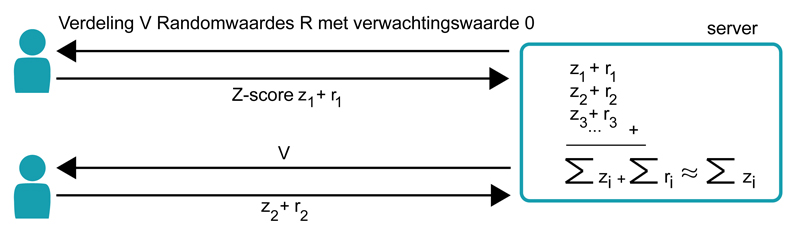
\includegraphics[scale=0.5]{fig/randomisatie}    
  \end{center}   
  \caption{Het basisprincipe bij een oplossing met randomisatie: bij een som over een grote groep gebruikers zal de som over de randomwaardes naar 0 gaan omdat de verwachtingswaarde van hun verdeling 0 is.}  
   \end{figure}
Om aan Singular Value Decomposition te doen heb je een user-feature matrix U en een item-feature matrix V nodig. De item-feature matrix V bereken je op basis van A’\^TA’. De waarden hiervan worden verkregen door het scalair product te nemen van de rijen van de matrix A’\^T en de kolommen van matrix A’. Als men deze som van producten over een groot aantal gebruikers neemt dan zal de waarde van de totale random verstoring naar 0 neigen. Dit komt omdat de random waarde gekozen is uit een verdeling met verwachtingswaarde 0. Uit de eigenwaarden van A’\^TA’. kan men dan de matrix V’ bepalen. De user-feature matrix U’ kan op een gelijkaardige manier benaderd worden met een som over de items. Deze aanpak wordt duidelijk nauwkeuriger naarmate er meer gebruikers en items zijn aangezien de impact van de willekeurig gekozen waarden uit de verdeling meer naar 0 zal neigen bij grotere sommaties.

Hoe meer verstoring, hoe meer privacy de gebruiker heeft maar ook hoe hoger de MAE-waarde en dus hoe slechter de aanbevelingen. Uit tests op de MovieLens en Jester dataset lijkt een keuze van randomwaarden uit de Gaussverdeling met standaarddeviatie 1 de beste resultaten te geven. Bij 100 gebruikers in de MovieLens dataset is de MAE zonder verstoring ongeveer 0.7146 en met verstoring 0.7964. Omdat de MovieLens database met een ratingsysteem werkt van 1 tot 5 sterren geeft het kleine verschil van 0.0818 in de MAE aan dat de kwaliteit van de aanbevelingen niet veel inboet door de aangebrachte verstoring.  De resultaten zijn bij nog meer gebruikers zoals verwacht zelfs nog beter. De Jester dataset gaf gelijkaardige resultaten.\\

Belangrijke kenmerken :
\begin{itemize}
 
\item Berekeningen van de aanbevelingen gebeuren op de server.
\end{itemize}
Voordelen : 
\begin{itemize}
\item Geen berekeningen aan client-zijde.
\end{itemize}
Nadelen:
\begin{itemize}
\item Biedt geen volledige privacy, de provider heeft nog steeds een idee in welke range de ratings liggen afhankelijk van de gebruikte verstoring. 
\item Werkt minder nauwkeurig met kleinere datasets.

\end{itemize}


\subsection{Op basis van verstoring door aggregatie}

\subsubsection{Aanpak door het gedistribueerd aggregeren van offline profielen door Shokri et al. \cite{LCA-CONF-2009-014}}

In tegenstelling tot de oplossing met randomisatie worden in deze methode niet de aparte ratings verstoord maar eerder de volledige profielen. De service provider berekent dan aanbevelingen op basis van deze verstoorde profielen. 

Een gebruiker heeft drie verschillende profielen. Het eerste profiel wordt bijgehouden aan de kant van de gebruiker en is enkel opgesteld met ratings geleverd door de gebruiker zelf. Dit profiel wordt nooit opgevraagd door de service provider. Een tweede profiel, het offline profiel genoemd, is een kopie van het eerste profiel uitgebreid met ratings uit offline profielen van andere gebruikers. Het online profiel dat bijgehouden wordt aan de kant van de server is eigenlijk een kopie van het offline profiel en haalt periodiek updates op van de client. Op basis van dit profiel zal de server zijn aanbevelingen berekenen.

Men kan gebruikers en items voorstellen als nodes in een graaf en ratings als verbindingen met gewicht tussen item en gebruiker. De client kan op een arbitraire manier contact met andere clients leggen. Bij een contact delen clients ratings van hun offline profielen. Hierbij kan de client vanzelfsprekend zijn eigen ratings behouden. Omdat deze interactie enkel tussen clients gebeurt heeft de server geen weet van welke clients onderling ratings delen. Hij weet dus ook niet welke ratings van het offline profiel van de gebruiker zelf  zijn en welke van een andere client afkomstig zijn.  Aangezien de clients onderling enkel gegevens van hun offline profiel delen geldt hetzelfde tussen gebruikers en is er dus ook een graad van user-user privacy. Het kan dan ook gebeuren dat de server items aanbeveelt die de gebruiker al beoordeeld heeft. Het is aan de clientapplicatie zelf om hierin te schiften.

\begin{figure}[htpb]   
    \label{Figuur::aggregatiefig}      
  \begin{center}    
 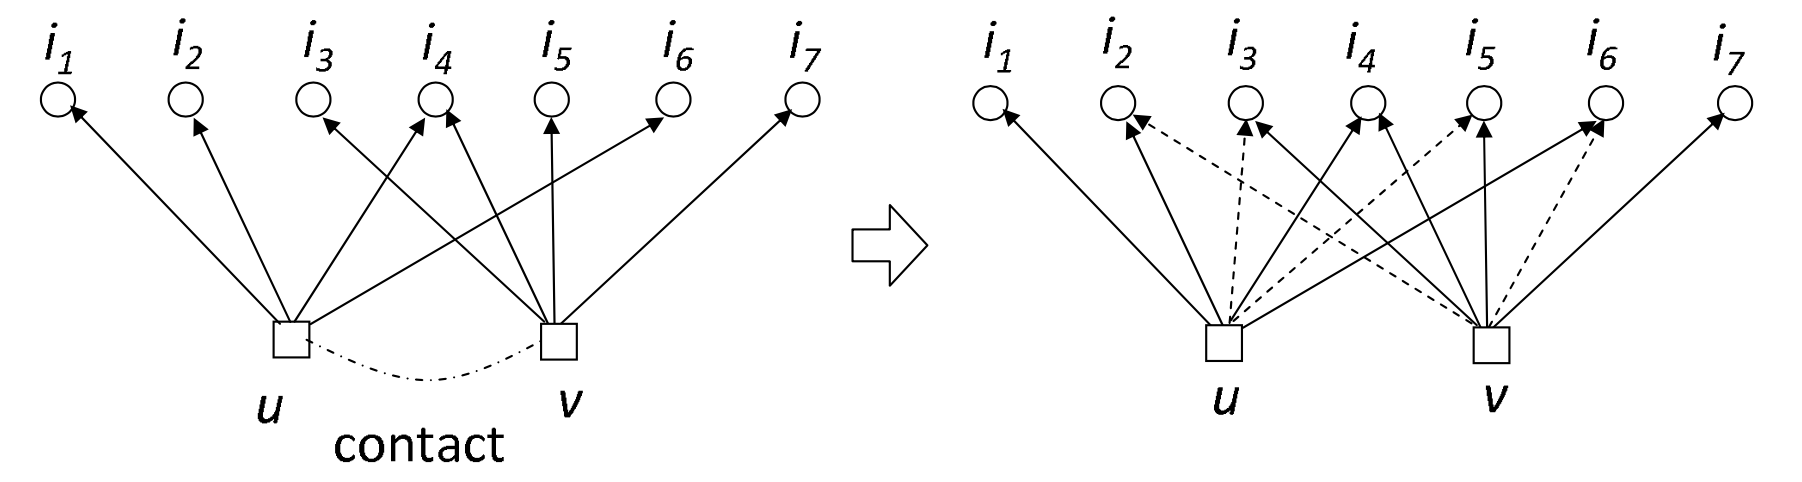
\includegraphics[scale=0.35]{fig/aggregatie}    
  \end{center}   
  \caption{Twee gebruikers wisselen ratings uit, uit \cite{LCA-CONF-2009-014}.}  
   \end{figure} 

Er moet vooraf bepaald worden welke ratings gedeeld worden tussen twee gebruikers en hoeveel. Shokri et al. geven hier verschillende opties voor. Alle ratings, een vast aantal ratings of het aantal ratings laten afhangen van de gelijkenis van twee gebruikers zijn mogelijkheden. De gelijkenis tussen twee gebruikers wordt privacyvriendelijk berekend met een methode van Lathia et al. \cite{lath}. Welke ratings worden gebruikt kan willekeurig gekozen worden of er kan een voorkeur gegeven worden aan de items die het minst geratet zijn over het hele systeem. Een onderzoek van Narayanan en Shmatikov \cite{nar} geeft aan dat een rating van een item, dat weinig beoordeeld is over alle users heen, sneller tot identificatie van een gebruiker kan leiden.  De optie om net deze ratings te delen tussen gebruikers heeft dus een positieve impact op de privacy.

De privacymaat wordt berekend op basis van de gelijkenis tussen de verstoorde online graaf en de originele graaf rekening houdende met aantal ratings per item. 
Als er gegevens met zes gebruikers per jaar uitgewisseld worden kan dit leiden naar een significante privacywinst van 0.68 de gebruiker naar de provider toe. bij een accuraatheidsverlies van 2\% . 


Belangrijke kenmerken :
\begin{itemize}
 
\item Deze methode is dan wel privacyvriendelijker dan de verstoring met randomisatie maar heeft toch zijn beperkingen.
\end{itemize}
Voordelen : 
\begin{itemize}
\item In tegenstelling tot de oplossing met randomisatie heeft hier de service provider geen idee welke items door de user zelf beoordeeld zijn. 
\item Weinig accuraatheidsverlies
\end{itemize}
Nadelen:
\begin{itemize}
\item Ratings van een offline profiel die lange tijd gelijk blijven hebben meer kans van die user zelf te zijn.
\item Het systeem krijgt de originele ratings van de gebruiker.

\end{itemize}


\subsection{Met behulp van cryptografische protocollen zonder server}

Hier is het uitgangspunt dat er geen vertrouwen meer nodig is in een provider indien de provider niet betrokken is bij het berekenen van aanbevelingen. Men werkt dus op een \textit{peer-to-peer} basis. De privacy van de gebruikers onderling wordt gerespecteerd door middel van secure multi-party computation.

Een voorbeeld is uitgewerkt door Hoens et al. 


\subsubsection{Aanpak op basis van cryptografische protocollen zonder server met behulp van een sociaal netwerk door Hoens et al. \cite{hoens2010private}}


Deze methode benut de vriendschapsrelaties op sociale netwerken. Men stelt dat aanbevelingen berekenen aan de hand van een sociaal netwerk betere resultaten levert dan een algemene aanpak omdat er gelijkenissen zijn tussen de smaak van een persoon en de smaak van zijn netwerk (vrienden, vrienden van vrienden,..). Een score voor een item wordt berekend door een gewogen gemiddelde te bepalen van de ratings van het netwerk van die persoon. Een optie is om hierbij de ratings van de gebruikers die dichter bij de gebruiker staan meer gewicht te geven. 
Tijdens de berekening van de score mag een gebruiker geen private informatie over het ratingsgedrag van een andere gebruiker te weten komen.

De vrienden van een gebruiker worden in deze context bekeken als zijn onmiddellijke kinderen in de boom. Eerst worden zijn onmiddellijke kinderen in de boom naar hun rating gevraagd om er een gewogen gemiddelde van te bepalen. Zij berekenen op hun beurt een rating op basis van een gewogen gemiddelde van hun kinderen enzovoort. Dit gebeurt tot de gewenste diepte bereikt is. De gebruiker kan eventueel zelf instellen hoe diep er mag worden afgedaald in de vriendschapsboom. Dit systeem heeft als nadeel dat bij \'e\'en interactieronde elke gebruiker online moet zijn op het sociaal netwerk.

Bij dit proces mag enkel de vragende gebruiker het voor hem berekende eindresultaat te weten komen. Andere tussenresultaten mogen noch door de aanvrager zelf of zijn netwerk leesbaar zijn. Om dit te bereiken worden verschillende cryptografische protocollen gebruikt. 

Homomorfische encryptie lijkt een logische keuze om de optelling/vermenigvuldiging te doen van de verschillende waarden vereist voor het berekenen van het gewogen gemiddelde. Daarnaast bestaat een (t,n)-threshold encryption, een encryptie die ervoor zorgt dat er medewerking van minstens t partijen nodig is om een waarde te decrypteren. Elke partij krijgt hierbij een deel van de sleutel. Omdat geen enkele partij volledig vertrouwd wordt zal het genereren van de sleutel ook moeten verdeeld worden tussen de partijen. Om aan homomorfische en threshold encryptie te voldoen kiest men ervoor gebruik te maken van het Paillier cryptosysteem. Voor de deling uit te voeren  bij de berekening van het gewogen gemiddelde wordt een nieuw protocol gebruikt.\\\\
Belangrijke kenmerken :
\begin{itemize}
 
\item Enkel bruikbaar voor Collaborative filtering
\item Berekeningen gebeuren bij de gebruiker zelf
\end{itemize}
Voordelen : 
\begin{itemize}
\item Gebruikt vriendschapsrelaties van sociale netwerken
\item Provider kan helemaal niets weten van private data gebruikers
\end{itemize}
Nadelen:
\begin{itemize}
\item Niet elk aanbevelingssysteem beschikt over een achterliggend sociaal netwerk.
\item Er gebeuren veel berekeningen bij de gebruiker. Dit is bij een mobiel toestel een belangrijk minpunt aangezien intensief cpugebruik liever vermeden wordt.
\item De oplossing gaat ervan uit dat andere gebruikers ook online zijn, wat voor vertragingen kan zorgen.
\end{itemize}




\subsection{Met behulp van cryptografische protocollen met server}
\subsubsection{Aanpak met behulp van cryptografische protocollen door Erkin et al \cite{ErkinBVL11}.}
\label{cryptoprotocollen}
Deze aanpak voert de verschillende stappen in het collaborative filteringproces privacyvriendelijk uit met behulp van verschillende protocollen. Om deze protocollen te kunnen uitvoeren genereert elke gebruiker eerst een sleutelpaar voor een Paillier en een DGK-cryptosysteem. Een eerste stap in dit proces is het bepalen van gelijkaardige gebruikers. Dit gebeurt aan de hand van de gekende Pearson-correlatie op ratings van items in een bepaalde range R. De Pearson-correlatie berekent gelijkenis tussen twee gebruikers aan de hand van de cosinus tussen hun smaakvectoren. De ratings in de range R noemt men de voorkeurenvector . De Pearson-correlatie \eqref{pearson} kan in 2 delen worden opgedeeld\cite{erkin:generating}:

\begin{equation}\label{pearson}sim_{A,B} = \frac{\sum_{j=0}^{R-1}(v_{(A,i)} - \bar{v}_A).(v_{(B,i)} - \bar{v}_B)}{\sqrt{\sum_{j=0}^{R-1} (v_{(A,j)} - \bar{v}_A)^2.\sum_{j=0}^{R-1} (v_{(B,j)} - \bar{v}_B)^2}} 
\end{equation}

\begin{equation}\label{similarity}sim_{A,B} = \sum_{i=0}^{R-1} C_{A,i}.C_{B,i} \end{equation}

\begin{equation}\label{c_value}
C_{X,i} = \frac{(v_{(X,i)} - \bar{v}_X)}{\sqrt{\sum_{j=0}^{R-1} (v_{(X,j)} - \bar{v}_X)^2}}\end{equation}
Zo kunnen twee gebruikers apart de C-waarden berekenen. De gebruiker die aanbevelingen vraagt encrypteert zijn voorkeurenvector met zijn public key. Dit stuurt hij naar de server die dit op zijn beurt doorstuurt naar een andere gebruiker. Door middel van het Paillier cryptosysteem kan deze de waarden van zijn voorkeurenvector respectievelijk vermenigvuldigen met de waarden voor de zelfde items van de voorkeurenvector van de aanvrager.  Van al deze producten wordt de som genomen \eqref{similarity} zoals in de Pearsoncorrelatie. De som geeft de gelijkenis weer tussen de twee gebruikers die nog steeds is ge\"encrypteerd met de publieke sleutel van de aanvrager. Deze waarde wordt dan teruggestuurd naar de server. De server voegt de ontvangen gelijkeniswaarden allemaal samen in een vector en voert hierop dan een aangepast protocol met de aanvrager. Dit aangepast protocol maakt gebruik van een DGK cryptosysteem in plaats van een Paillier cryptosysteem voor effici\"entieredenen. Het resultaat is een geëncrypteerde vector van enen en nullen die aangeeft of  de gelijkeniswaarde tussen de aanvrager en de respectievelijke gebruiker boven een bepaalde ondergrens ligt. De server stuurt deze naar de gebruiker zodat hij zijn ratings kan vermenigvuldigen met deze waarde en terugsturen. Hierop maakt de server de som van de ratings over alle gelijkaardige gebruikers en stuurt deze naar de aanvrager die de som decrypteert en er een gemiddelde van berekent.

Met behulp van dit protocol worden enkel de ratings van gelijkaardige gebruikers gebruikt. Geen enkele entiteit kan de gelijkenis tussen twee gebruikers bepalen.\\



Belangrijke kenmerken :
\begin{itemize}

\item Berekeningen van de aanbevelingen gebeuren door de server en de client.
\end{itemize}
Voordelen : 
\begin{itemize}
\item Dankzij diverse cryptografische protocollen is dit een volledig privacyvriendelijke oplossing in een statische setting
\end{itemize}
Nadelen:
\begin{itemize}
\item Bij een dynamische userdatabase kan deze oplossing gegevens van de gebruikers lekken. Als een zelfde gebruiker tweemaal aanbevelingen vraagt met de tweede maal \'e\'en gebruiker meer kan hij afleiden of deze extra gebruiker een gelijkaardige smaak heeft als hijzelf, afhankelijk van of deze gebruiker een invloed heeft op zijn aanbevelingen of niet. Men spreekt over een "\emph{new group attack}" \cite{kononchuk2013privacy}.
\item Cryptografie zorgt voor een overhead.

\end{itemize}


\subsection{Conclusie onderzoek}

Nu er van de belangrijkste soorten oplossingen zijn doorgelicht, kan er besloten worden in welke richting we verderwerken. Een eerste optie met behulp van randomisatie leek op het eerste zicht erg interessant omdat deze heel weinig berekeningen aan de clientkant vraagt, wat natuurlijk een pluspunt is bij mobiele toestellen. Helaas werkt dit systeem niet goed bij lage gebruikersaantallen en kan het informatie lekken aan de service provider afhankelijk van de gekozen verdeling. Daar heeft de verstoring met behulp van aggregatie geen last van. Deze biedt qua privacy wel deniability of preferences aan de user maar geeft de provider wel toegang tot originele beoordelingen van de gebruiker. Als Narayan en Schmatikov in \cite{Narayanan2008} anonieme profielen kunnen linken met users met maar een beperkte kennis over deze gebruiker, lijkt het maar een kleine stap om uit het aangegeven verstoorde profiel de juiste ratings bij een gebruiker te plaatsen. Zeker indien er maar wordt geaggregeerd met een beperkt aantal andere gebruikersprofielen zoals in \cite{LCA-CONF-2009-014} beschreven. Hoewel de oplossing op basis van een sociaal netwerk erg privacyvriendelijk is, is ze niet echt flexibel. Ze vereist dat andere gebruikers online zijn en ook actief meewerken aan het protocol. Door het \emph{peer-to-peer} karakter van deze werkwijze zijn de clients verplicht om alle berekeningen zelf te doen. Het is duidelijk dat deze eigenschappen in een mobiele setting niet gewenst zijn.
Bij de oplossing met anonimisatie heeft de clientapplicatie daarentegen weinig werk. Het stuurt de beoordelingen rechtstreeks naar de filterentiteit, die moet vertrouwd worden. De anonimisatie die gebeurt in het user-user collaborative filtering systeem of de kennis-gebaseerde versie voldoet niet om volledig privacyvriendelijk te zijn zoals aangegeven in \ref{onterecht_vertrouwen}. De meest privacyvriendelijke oplossing lijkt de methode met behulp van cryptografische protocollen en een server. Het systeem werkt er volledig privacyvriendelijk in een statische setting. Uit verder onderzoek blijkt dat dezelfde auteur ook een paper uitbracht in november 2013 \cite{ZErkinDyn} die een erg gelijkaardige oplossing aanbiedt die ook privacyvriendelijk is in een dynamische setting. Deze methode heeft als extra voordeel dat de gebruikersapplicatie relatief weinig berekeningen hoeft te doen. Het enige minpunt is dat de berekeningen aan de serverkant erg zwaar zijn door de cryptografische protocollen. We besluiten voor deze werkwijze te kiezen en deze verder te optimaliseren in een mobiele setting in hoofdstuk \ref{privacy_opl}.
%\begin{figure}[htb]
%\begin{center}
%optioneel om evt wat witruimte van je figuur af te snoepen
%\vspace{-.3cm}
% 
\includegraphics[keepaspectratio,width=0.5\textwidth]{fig/ruglogo}
% analoog
%\vspace{-0.6cm}
 %\caption{Het RUG logo}
 %\label{fig:ruglogo}
%analoog
%\vspace{-.6cm}
%\end{center}
%\end{figure}


\chapter{Privacyvriendelijk aanbevelingssysteem voor mobiele toestellen}
\label{privacy_opl}




\section{Inleiding}
De keuze voor vertrekpunt van onze oplossing viel op de werkwijze van Z. Erkin, T. Veugen en R.L. Lagendijk beschreven in "Privacy-preserving recommender systems in dynamic environments \cite{ZErkinDyn}". Deze laat user-user collaborative filtering toe op een privacyvriendelijke manier. Kort samengevat gaat deze een voorspelling van een beoordeling van een gebruiker A doen door de gemiddelde rating te nemen van gebruikers die een gelijkenis hebben met A die hoger ligt dan een bepaalde drempelwaarde. De basis van de werkwijze uit \cite{ZErkinDyn} is gebleven, maar er werden eigen accenten gelegd rekening houdend met de mobiele setting. \\Net als het besproken systeem in paragraaf \ref{cryptoprotocollen} maakt dit systeem gebruik van cryptografische protocollen met behulp van een Paillier en een DGK-cryptosysteem. Technieken gebaseerd op cryptografie hebben het voordeel dat de privacy bewijsbaar is als de gebruikersdata wordt ge\"encrypteerd. De service provider kan dan door de homomorfische eigenschappen van de cryptosystemen zijn taken verrichten zonder toegang te krijgen tot deze data. Buiten de gebruikersvoorkeuren worden ook de gelijkeniswaarden tussen gebruikers en de uiteindelijke aanbevelingen afgeschermd van de service provider door encryptie.\\ Om problemen te voorkomen in een dynamische setting zoals in \ref{cryptoprotocollen} wordt ook de informatie verminderd waarover de provider beschikt bij herhaaldelijke aanvragen van aanbevelingen. Dit wordt verwezenlijkt door gebruik te maken van een tweede server, een server die onafhankelijk moet zijn van de server van de service provider. Deze tweede server wordt in dit naslagwerk ook vernoemd als controle server. De controle server gedraagt zich als privacy provider. Deze rol kan bijvoorbeeld vervuld worden door de overheid of een ander commercieel bedrijf. Het gebruik ervan zou opgelegd kunnen worden door de overheid in bepaalde privacygevoelige sectoren zoals bijvoorbeeld een systeem gebaseerd op medische data. Er wordt vanuit gegaan dat beide servers optreden in een "\emph{semi-honest}" model, wat betekent dat ze betrouwbaar genoeg zijn om het onderling protocol in volgorde uit te voeren. \\ Beide servers beschikken over een Paillier-sleutelpaar, hiernaast heeft de controleserver ook een DGK-sleutelpaar. Voor de Paillier-encryptie werd er beroep gedaan op een zelfs aangepaste versie op basis van code uit The Homomorphic Encryption Project (THEP https://code.google.com/p/thep/). De DGK-encryptie gebeurde met code uit https://github.com/winderif/PTSwithGC/tree/master/Crypto. Zoals eerder vermeld werd er gekozen om de clientapplicatie uit te werken in Android en deze communiceert met de Javaservers via het HTTP-protocol. We gebruiken de MovieLens database, de standaard voor het testen van aanbevelingssystemen.

\section{Werking}


\subsection{Diagram van het hoofdprotocol}

Het volgend sequentiediagram geeft de communicatie weer tussen de clientapplicaties en de twee servers als een gebruiker aanbevelingen vraagt. De paragrafen waar de onderdelen ervan besproken worden staan links aangegeven. Functies, protocollen en taken staan in het zwart aangegeven, attributen in het blauw. De berekeningen op de aanbevelingsserver gebeuren in het gesloten Pailliersysteem getekend met publieke sleutel S2 zodat de server geen persoonlijke data kan lezen.

Alvorens het aanvragen van aanbevelingen slaat een gebruiker zijn beoordelingen en voorkeuren op en stuurt ze dan samen in zijn profiel naar de recommenderserver (\ref{voor_aanvraag}). Eens user 1 aanbevelingen vraagt is de eerste stap de gelijkenisfactor berekenen tussen user 1 en de andere users Ux. Dit gebeurt door de aanbevelingsserver in paragraaf \ref{similarities}.  Daarna gaat de server met het thresholdprotocol (\ref{threshold}) na of deze ge\"encrypteerde waarden boven een drempelwaarde liggen. Nu bezit de recommender een ge\"encrypteerde bit per gebruiker die aangeeft of dit wel (1) of niet (0) het geval is. Hierop starten de recommender en de privacy provider een nieuw protocol waarbij de controleserver een deel van de gebruikers selecteert die kunnen meedoen aan het protocol (\ref{selection}). De resultaatbits hiervan geven aan of de ratings van respectievelijke gebruiker zullen worden meegeteld in het berekenen van de aanbevelingen. Het multiplicationprotocol (\ref{multiplication}) vermenigvuldigt deze gebruikerbits met zijn overeenkomstige ratings. Daarna wordt de som van de ratings per item genomen over alle gebruikers heen in paragraaf \ref{sumoverallusers} en wordt het resultaat privacyvriendelijk naar de gebruiker gebracht (\ref{result}).
\begin{center}
\begin{figure}[htpb]   
    \label{Figuur::hoofdprotocol}      
   
\centering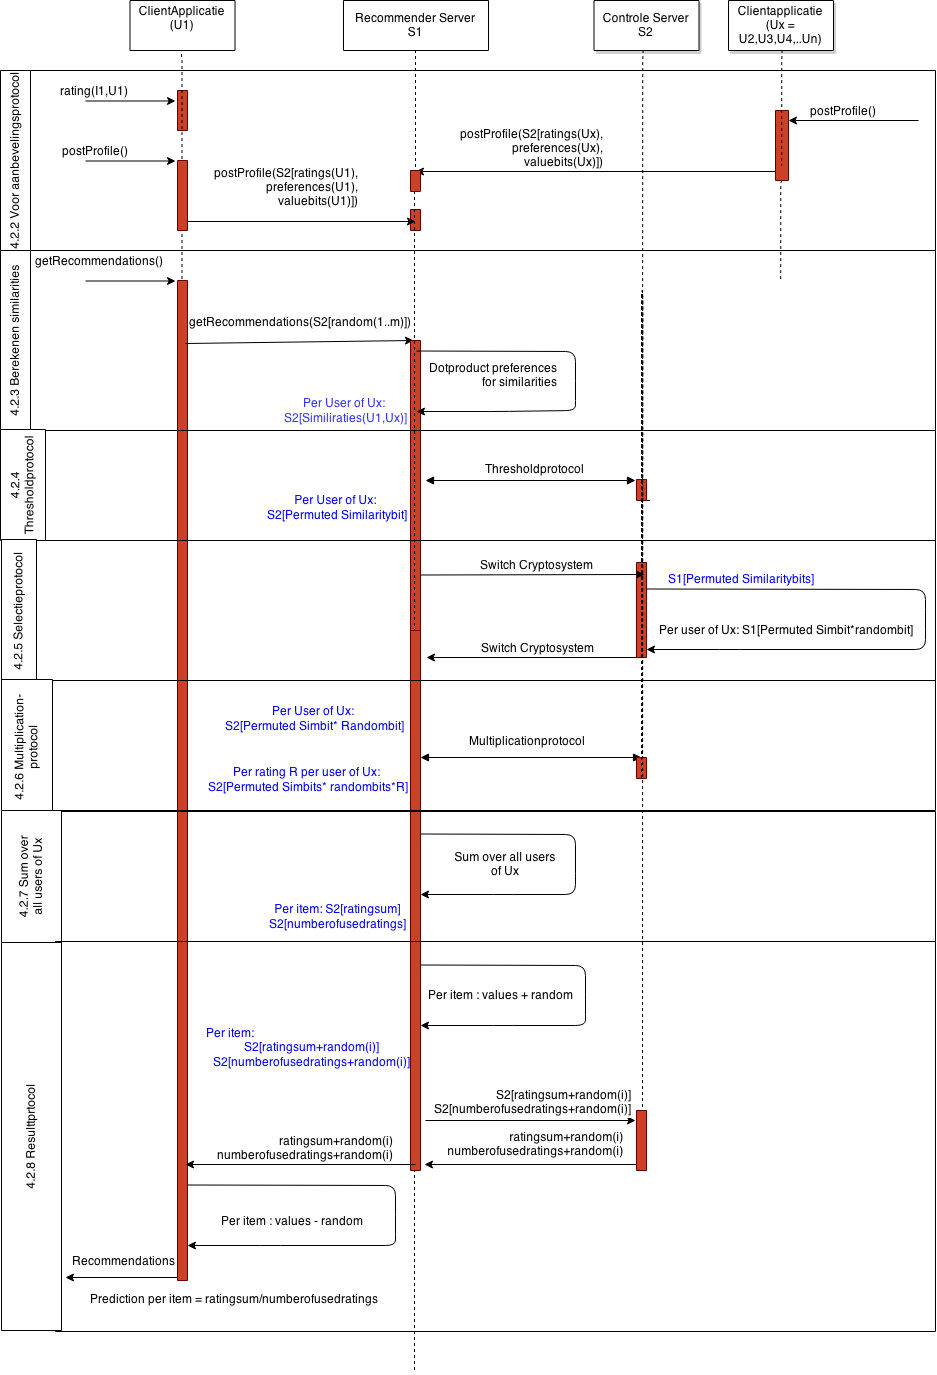
\includegraphics[width=1.0\textwidth,keepaspectratio]{fig/hoofdprotocol_privacy}    
   
   \end{figure}
   \end{center}


\subsection{Voor een aanbevelingsaanvraag}
\label{voor_aanvraag}
Voor een aanbevelingsaanvraag zal de gebruiker verschillende items beoordelen. De ratings worden lokaal bijgehouden in de Androidapplicatie in een SQLiteDatabase. Ze worden daarna voor het sturen van het profiel ge\"encrypteerd met de publieke sleutel van het Pailliersysteem van de controleserver en naar de recommenderserver gestuurd.

\begin{figure}[htpb]   
    \label{Figuur::all_items}      
  \begin{center}    
 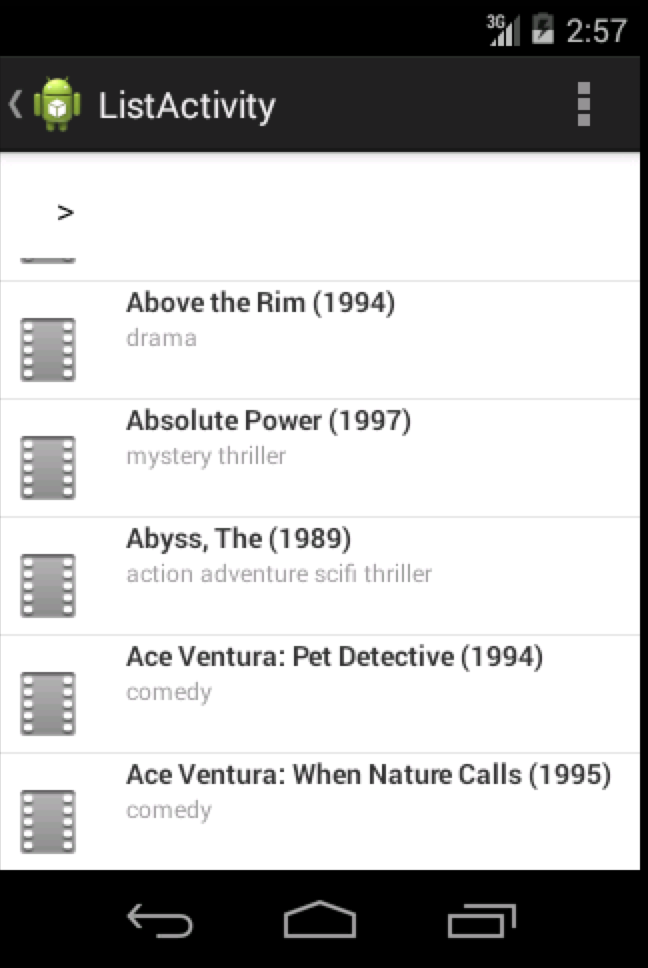
\includegraphics[scale=0.5]{fig/all_items}    
  \end{center}   
  \caption{De gebruiker krijgt de lijst met films te zien uit de MovieLensdatabase}  
   \end{figure}
   
   \begin{figure}[htpb]   
    \label{Figuur::rate_item}      
  \begin{center}    
 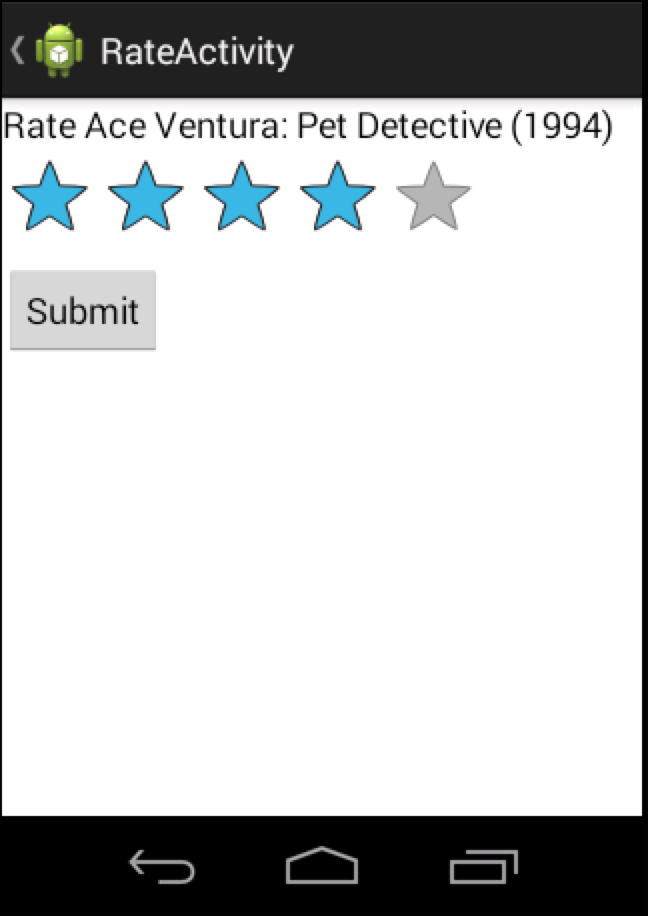
\includegraphics[scale=0.5]{fig/rate_item}    
  \end{center}   
  \caption{De gebruiker beoordeelt een film.}  
   \end{figure}
Om de gelijkenis te berekenen tussen twee gebruikers wordt er dezelfde methode gebruikt als in \ref{cryptoprotocollen} en wordt de Pearson-co\"efficient dus opgesplitst \eqref{similarity}.\\ 
Per gebruiker moeten dus de \emph{preferences} of C-waarden $C_{X,i}$ bepaald worden. De preferences worden bepaald op basis van de ratings van een bepaalde deelverzameling van de items. Deze deelverzameling wordt het best bepaald door items te nemen die door het gros van de gebruikers beoordeeld zijn. Om deze lijst dynamisch te bepalen zou de recommenderserver moeten weten hoeveel gebruikers een bepaald item ge\"evalueerd hebben. Dat kan niet dynamisch bepaald worden gezien het volledig privacyvriendelijk karakter van dit systeem. Hierdoor mag de server niet weten welke gebruiker welk item beoordeeld heeft, zelfs al weet de server de waarde van de beoordeling niet.
Dit zou contact kunnen verraden tussen een user en een item, bijvoorbeeld dat een persoon naar een restaurant geweest is.
Het systeem zou met deze data zelfs een smakenprofiel van een gebruiker opzetten. Een oplossing voor dit probleem is de deelverzameling vast kiezen en eventueel bij het eerste gebruik aan de gebruiker vragen deze lijst te evalueren, zonder hem te verplichten een bepaald item te raten. Deze deelverzameling zou dan best opgesteld worden uit items waarover de mening van de gebruikers verdeeld is en niet diegene die de meeste users goed of slecht vinden. Om deze complicaties te vermijden gebruiken we in onze testapplicatie de ratings van alle items als preferences.

De  $\bar{v}_X$ en $\sqrt{\sum_{j=0}^{M-1} (v_{(X,j)} - \bar{v}_X)^2}$ waarden zijn voor elke C-waarde gelijk. Dit betekent dat je de C-waarde eventueel ook aan de kant van de server zou kunnen berekenen en voor de deling in het Pailliersysteem gebruik maken van een protocol als \cite{VeugenEID}. Dit lijkt niet zo effici\"ent en er werd besloten de berekening van de C-waarden te doen op de client en ge\"encrypteerd mee te sturen in het profiel.
\begin{figure}[htpb]   
    \label{Figuur::upload_profile}      
  \begin{center}    
 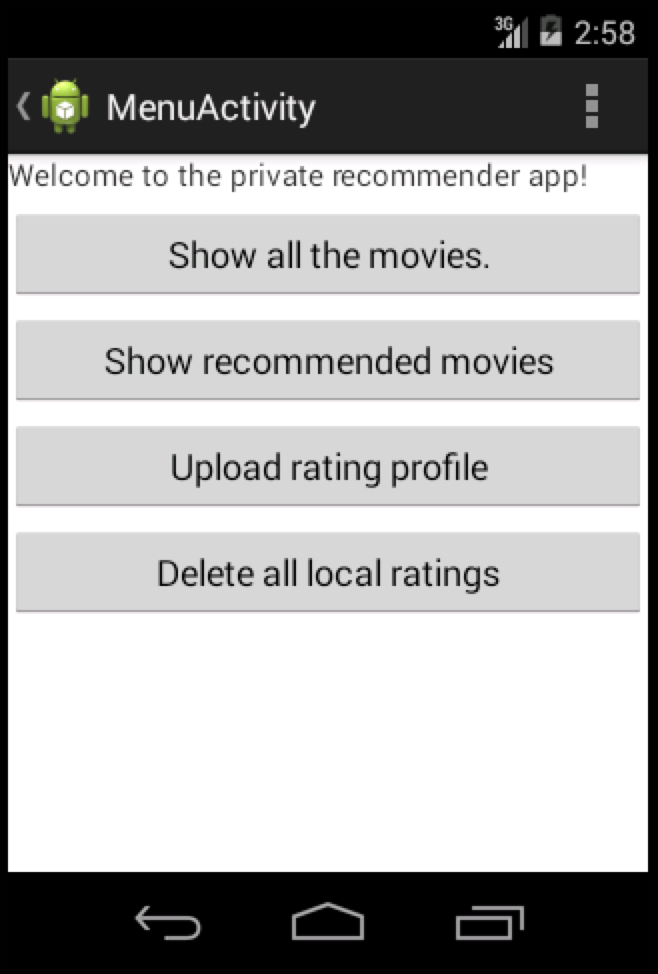
\includegraphics[scale=0.5]{fig/upload_profile}    
  \end{center}   
  \caption{Het menu van de testapplicatie. De gebruiker kan zijn profiel uploaden wanneer hij wil.}  
   \end{figure}
Naast de lijsten van de ratings en de preferences geven we ook nog een lijst ge\"encrypteerde bits mee die aangeven of een item wel (1) of niet (0) beoordeeld is door deze gebruiker. Dit lijkt redundante informatie maar dit kunnen we gebruiken als we moeten optellen hoeveel (ingevulde) ratings er werden opgeteld.  Dat komt omdat als we het profiel naar de server sturen ook "ratings" moeten doorsturen van items die de persoon nog niet beoordeeld heeft. Dit om te verbergen welke items de persoon ge\"evalueerd heeft. Dit is een uitbreiding op de theoretische paper \cite{ZErkinDyn} waar er vanuit gegaan wordt dat alle ratings ingevuld zijn.  We sturen ook best de waarden van alle items mee, anders zitten er C-waarden in de databank op de server berekend op verourde $\bar{v}_X$ en $\sqrt{\sum_{j=0}^{M-1} (v_{(X,j)} - \bar{v}_X)^2}$ waarden. Deze manier geeft ook de garantie op de hoogste privacy.

We geven ook de gebruiker de keuze wanneer hij zijn profiel uploadt en hij kan ook zijn lokale ratings leegmaken. Dit geeft hem meer controle over zijn profiel en laat hem toe om zijn profiel eerst leeg te maken en dan up te loaden. Zo heeft de aanbevelingsserver geen enkele ge\"encrypteerde beoordeling meer staan van deze gebruiker, tenzij hij natuurlijk backups nam. Het bespaart ook data-overdracht en processortijd als de upload niet bij elke rating gebeurt.

Nu moet er de keuze gemaakt worden wanneer de encryptie gebeurt. De encryptie gebeurt optimaal op het moment dat het profiel wordt gestuurd naar de aanbevelingsserver en niet alvorens de rating in de databank wordt geplaatst. Dit is aan de ene kant logisch aangezien ook de C-waarden dan het best berekend worden met de laatste waarden, maar zorgt er ook voor dat alle ge\"encrypteerde waarden telkens anders zijn zodat de server niet kan zien welke waarden veranderd zijn ten opzichte van een vorige rating dankzij de semantische veiligheid van het Paillier-cryptosysteem.
\subsection{Berekenen van gelijkeniswaarden tussen gebruikers}
\label{similarities}

Het berekenen van gelijkeniswaarden gebeurt zoals eerder aangegeven door de Pearson-co\"efficient. Aangezien de ge\"encrypteerde C-waarden hiervoor al op de clientapplicatie worden berekend hoeven we enkel nog het scalair product te nemen van deze waarden met de formule $sim_{A,B} = \sum_{i=0}^{R-1} C_{A,i}.C_{B,i}$ uit paragraaf \ref{cryptoprotocollen}. Ge\"encrypteerd met de publieke sleutel van de controleserver wordt dit (naar \cite{ZErkinDyn}):
\begin{equation}\label{similarity}[sim_{A,B}]_2 = \prod_{i=0}^{R-1} [C_{A,i}]_2 \otimes [C_{B,i}]_2 \end{equation}

De som wordt omgezet in een product dankzij de homomorfe eigenschappen van het Pailliersysteem (\ref{paillier}). Het product tussen twee ge\"encrypteerde waarden uitrekenen, hier aangegeven met  $\otimes$, is niet zo eenvoudig. Hiervoor wordt dezelfde werkwijze gebruikt als in het multiplicatieprotocol (\ref{multiplication}).
\subsection{Thresholdprotocol}
\label{threshold}

Dit protocol uit Privacy-Preserving Face Recognition \cite{facerecog} laat toe om twee ge\"encrypteerde waarden $[a]_2$ en $[b]_2$ te vergelijken met als resultaat een ge\"encrypteerde bit die $[1]_2$ is als $a \geq b$ als en $[0]_2$ is als $a < b$. We gebruiken dit om een gelijkeniswaarde sim tussen de gebruikers te vergelijken met een drempelwaarde d. De drempelwaarde kan de service provider zelf vrij kiezen. Welke drempelwaarde de beste is, is afhankelijk van de dataset. De provider encrypteert de waarde met de publieke Pailliersleutel van de controleserver zodat het besproken protocol kan worden toegepast.

Het aanbevelingssysteem berekent eerst $[z]_2$
\begin{equation}
[z]_2 = [2^l + sim - d]_2 =[2^l]_2.[sim]_2.[d]_2  \end{equation}

Als we het binair bekijken geeft de grootste bit van z inderdaad de verhouding van sim ten opzichte van d aan.
Deze bit is de $l$-de bit (geteld vanaf rechts beginnend bij 0) en wordt $z_l$ genoemd. De waarde van $z_l$ kan als volgt berekend worden.
\begin{equation}
\label{zl}
z_l = 2^{-l}.(z-(z\mod 2^l)) \end{equation}

Hier worden eerst alle bits behalve de meest linkse op 0 gezet door $z-(z\mod 2^l)$ en wordt de bit dan naar rechts geschoven door te vermenigvuldigen met $2^{-l}$. De aanbevelingsserver beschikt niet over $[z\mod 2^l]_2$ en zal dus hulp moeten vragen aan de controleserver, die de waarde van z niet mag kennen. De waarde van z wordt dus eerst vermomd met een randomwaarde r.
\begin{equation}
[c]_2= [z+r]_2 = [z]_2.[r]_2 \end{equation}
De c-waarde wordt dan naar de controleserver gestuurd die c uitpakt en $c\mod 2^l$ berekent. Hij stuurt $c\mod 2^l$ op twee manieren terug. E\'en maal geheel Paillierge\"encrypteerd en \'e\'enmaal opgesplitst in bits DGKge\"encrypteerd (zie straks). Omdat $[c]_2= [z+r]_2 = [z]_2.[r]_2$ geldt dat:

\begin{equation}
\label{zmod}z\mod 2^l = (c\mod 2^l - r\mod 2^l)\mod 2^l \end{equation}
Dus afhankelijk van of $c\mod 2^l < r\mod 2^l$ moeten we bij $c\mod 2^l - r\mod 2^l$ wel of niet $2^l$ bijtellen. Dit is het zogenaamde miljonairsprobleem van Yao waarbij twee partijen beschikken over een getal dat ze niet aan de andere partij bekend willen maken maar ze willen wel weten welke het grootste is. Hiervoor worden de $e_i$-bits (i staat voor de plaats van de bit) berekend, waarvoor we de bits van $c \mod2^l$ en $r \mod 2^l$ gebruiken. Er wordt voor dit subprotocol een DGKsysteem gebruikt voor effici\"entieredenen.  De recommender kiest een s-waarde 1 of -1 die aangeeft in welke richting de vergelijking gebeurt. De DGKencryptie geven we aan met dubbele haakjes [[]].
\begin{equation}
[[e_i]]=[[sim_i - r_i + s+ 3.\sum_{j=i+1}^{l-1}(sim_j \oplus r_j)]]
\end{equation}
Eens alle $e_i$-bits berekend werden kunnen we de $\gamma$-bit bepalen. Deze is 0 als er \'e\'en $e_i$-bit 0 is en anders 1.
\begin{itemize}
 
\item Als s=1 is en $\gamma = 1$  dan is $sim > r$, is $\gamma=0$ dan is $sim< r$.
\item  Als s=-1 is en $\gamma = 1$  dan is $sim < r$, is $\gamma=0$ dan is $sim> r$.
\end{itemize}   Het aanbevelingssysteem stuurt de $e_i$-bits gepermuteerd naar de controleserver. Die decrypteert ze en berekent de $\gamma$-bit, hij weet niet wat deze betekent aangezien hij de waarde van s niet kent. Hij encrypteert de $\gamma$-bit met zijn publieke Pailliersleutel en stuurt deze terug naar de recommenderserver. De recommenderserver kent de waarde van s en weet dus wat deze ge\"encrypteerde $\gamma$-bit betekent. Hij kan dus $[\lambda]_2$ berekenen de bit die aangeeft of $cmod2^l < rmod2^l$ en dus of $2^l$ moet opgeteld worden bij $cmod2^l - rmod2^l$ in \ref{zmod}.
Als $s = 1$ heeft  $\lambda=1$ de omgekeerde bitwaarde als $\gamma$. De omgekeerde bitwaarde kan berekend worden door  $\gamma \oplus 1$. De XOR functie wordt nagebootst met $[a \oplus b]_2= [a + b - 2ab]_2 = [a]_2*[b]_2*[a]_2^{-2b}$ Als $s =-1$ is $\lambda = \gamma$. Hierdoor heeft de recommender dus genoeg info om \ref{zmod} te berekenen en daarna \ref{zl}.

\subsection{Selectie maken van gebruikers}
\label{selection}
Na het meerdere keren aanroepen van het aanbevelingssysteem, zou het systeem of een gebruiker kunnen afleiden welke invloed de data van bepaalde gebruikers heeft op de aanbevelingen. Dit heet een new group attack en is eerder al vernoemd in \ref{cryptoprotocollen}. Om een new group attack tegen te gaan wordt er door de controleserver een selectie van gebruikers gemaakt die kunnen deelnemen aan het protocol. De recommender mag deze selectie dus niet kennen. Om een selectie te laten maken zou de recommender de gelijkenisbits naar de controleserver moeten sturen. De bits zijn nog ge\"encrypteerd met de publieke sleutel van de controleserver, die deze bits niet mag kennen. Om dit op te lossen worden er randomgetallen $[\rho_i]_1$ bij de ge\"encrypteerde simbits geteld. Het negatieve randomgetal wordt zelf ook meegestuurd, ge\"encrypteerd met de publieke sleutel van de recommenderserver. Zo kan de controleserver $[sim_i+\rho_i]_2$ decrypteren met zijn eigen private sleutel. Deze som encrypteert hij dan weer met de publieke sleutel van de recommenderserver. Op die manier kan hij de randomwaarde hiervan aftrekken met het Pailliersysteem $[sim_i+\rho_i-\rho_i]_1$ en de originele gelijkenisbits verkrijgen. De controleserver maakt nu een tabel aan met bits met evenveel 1-waarden als gebruikers die hij wil betrekken in het protocol. In \cite{ZErkinDyn} wordt een waarde $n/2$ voorgesteld voor voldoende privacy. De server vermenigvuldigt deze bits met de gelijkenisbits en stuurt het resultaat terug naar de aanbevelingsserver. Hierbij wordt nogmaals gewisseld van cryptosysteem zoals bij het heensturen van de bits. Hier volgt een kijk in de code die aangeeft wat er gebeurt op de controleserver als deze een selectie moet maken. Er werd een extra constructor gemaakt voor EncryptedInteger uit het Pailliercryptosysteem uit THEP. De constructor waar de Pailliersleutel als eerste argument gegeven wordt cree\"ert een EncryptedIntegerobject op basis van een ge\"encrypteerd BigIntegerobject. De tweede en originele constructor, waar de Pailliersleutel als tweede argument wordt gegeven zal een plaintext BigIntegerobject encrypteren en op basis hiervan een EncryptedIntegerobject maken.

\begin{verbatim}
public DeltaDAO exchangeDeltas(DeltaDAO d) throws Exception {...
    //Afhankelijk van het procent van de gebruikers worden er bits bepaald 
    // en door elkaar geschud
	...
    	shuffleArray(bi);
    	List<BigInteger> rands = new ArrayList<BigInteger>();
    for(int j=0;j< d.getDeltas().size();j++){
    // De controleserver decrypteert de waarde van (de bit + de toegevoegde 
    // randomwaarde) door de recommenderserver.
       	EncryptedInteger inBit = new EncryptedInteger(
       		PaillierResource.pubKey,d.getDeltas().get(j));
       	BigInteger decryptInBit =  inBit.decrypt(PaillierResource.privKey);
    // De controleserver encrypteert de gedecrypteerde waarde met de publieke sleutel
    // van de recommenderserver zodat hij er de negatieve randomwaarde kan bij 
    // optellen en de ge\"encrypteerde versie van de originele bit verkrijgt.
    		EncryptedInteger randEncRec = new 
        		EncryptedInteger(pubKeyRecommenderServer,d.getRandoms().get(j));
      	EncryptedInteger bEncRec = new EncryptedInteger(decryptInBit,
      		pubKeyRecommenderServer);
        	bEncRec= bEncRec.add(randEncRec);
    // Hij vermenigvuldigt de random gepermuteerde bit met de originele bit en 
    // voegt er een nieuwe randomwaarde bij om een tweede maal van cryptosysteem 
    // te wisselen.
       	bEncRec = bEncRec.multiply(bi[j]);
        BigInteger random = new BigInteger(10,random);
       	EncryptedInteger rEnc = new EncryptedInteger(random,pubKeyRecommenderServer);
        	bEncRec = bEncRec.add(rEnc);
       	d.getDeltas().set(j, bEncRec.getCipherVal());
       	random =random.multiply(new BigInteger("-1");
       	rands.add(new EncryptedInteger(random),PaillierResource.pubKey).getCipherVal());        
   	}
    	d.setRandoms(rands);
    	return d;        
}
\end{verbatim}
\subsection{Multiplicatieprotocol}
\label{multiplication} 
Hier vermenigvuldigt de recommenderserver de ratings en bitvalues van de gebruiker met hun overeenkomstige resultaatbits uit \ref{selection} die aangeven of hun beoordeling worden opgenomen in het protocol. De vermenigvuldiging van twee ge\"encrypteerde waarden zit niet standaard in het Pailliercryptosysteem. Dit wordt opgelost door dit eenvoudig subprotocol \cite{erkin:generating}. De aanbevelingsserver bepaalt per vermenigvuldiging eerst twee random getallen $r_1$ en $r_2$ die hij aftrekt van de respectievelijke bits en zo $[sim_x - r_1]_2$ en $[rating_y - r_2]_2$ bepaalt. Hij stuurt deze naar de controleserver die deze decrypteert, vermenigvuldigt, weer encrypteert met zijn publieke sleutel en terugstuurt. Zo kan de recommenderserver het resultaat van de vermenigvuldiging berekenen door:

\begin{equation}
[sim_x.rating_y]_2=[(sim_x-r_1).(rating_y-r_2) + sim_x.r_2 + rating_y.r_1 - r_1.r_2]_2
\end{equation}
\begin{equation}
[sim_x.rating_y]_2= [(sim_x-r_1).(rating_y-r_2)]_2 . [sim_x]_2^{r_2} . [rating_y]_2^{r_1}.[-r_1.r_2]_2
\end{equation}
Deze berekeningen zijn allemaal mogelijk in het Pailiercryptosysteem.
\subsection{Som over alle gebruikers heen}
\label{sumoverallusers}

In dit deel worden de waarden van de ratings en bitvalues (beide vermenigvuldigd met de resultaatbit) samengeteld per item over alle gebruikers heen. Op deze manier beschikt de recommenderserver over een ge\"encrypteerde som van de ratings die worden meegeteld en het ge\"encrypteerde aantal ratings dat wordt meegeteld.
\subsection{Resultaatprotocol}
\label{result}

\begin{center} 
\centering 
 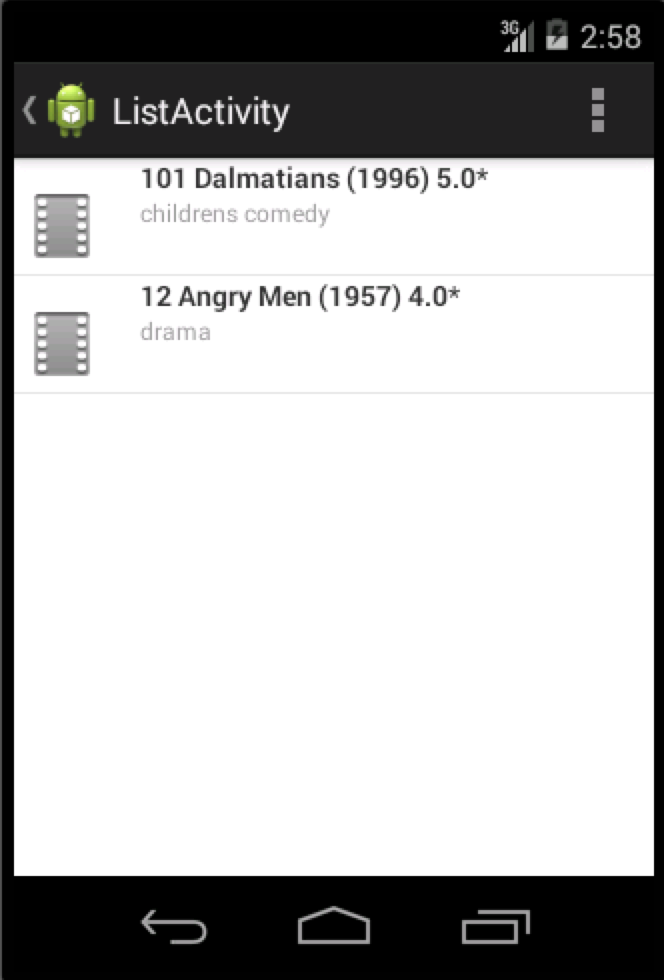
\includegraphics[scale=0.5]{fig/recommendations}    
    \label{Figuur::recommendations}   
    \captionof{figure}{De gebruiker krijgt een lijst met aanbevelingen en een voorspelling van het aantal sterren dat hij aan deze film zou geven.}   
\end{center}

   
Het resultaatprotocol zorgt ervoor dat de twee berekende waarden per item uit \ref{sumoverallusers}, de som der ratings en het aantal, op een privacyvriendelijke manier bij de aanvrager terechtkomen. Bij het aanvragen van aanbevelingen gaf de clientapplicatie randomwaarden mee. Deze worden bij de waarden geteld en naar de controleserver gestuurd die ze decrypteert en terugstuurt naar de recommender, die op zijn beurt ze gewoon teruggeeft aan de gebruiker. De gebruiker trekt er zijn gegenereerde randomwaarden van af en verkrijgt de originele waarden. Hierop bepaalt hij de gemiddelde rating van gelijkaardige gebruikers door ze eenvoudigweg te delen. De clientapplicatie is wel verantwoordelijk om de items die reeds door de gebruiker zelf zijn beoordeeld uit de resultaten te filteren.

\chapter{Resultaten}
Hier wordt besproken hoe het uitgewerkte aanbevelingssysteem scoort op de drie belangrijke pijlers: nauwkeurigheid, privacy en performantie.
\section{Privacy}
Deze oplossing biedt veruit de beste privacybescherming uit al de besproken mogelijkheden. Beide servers doen het merendeel van de berekeningen in het ge\"encrypteerd Paillier- of DGKdomein. In de gevallen waar een server rekent met plaintext is deze dermate verstoord zodat deze server de originele waarde niet kan kennen. Het Pailliercryptosysteem en het DGKsysteem worden als semantisch veilig beschouwd. Dit betekent dat het niet \emph{feasible} of computationeel haalbaar is dat er extra informatie kan gehaald worden over de plaintext uit de ciphertext. Homomorfische systemen als Paillier en DGK kampen wel met het probleem dat een aanvaller die een \emph{man-in-the-middle attack} uitvoert de plaintekst kan vermenigvuldigen met een gewenste waarde en kan sturen naar de ontvanger. De aanvaller kan de waarden dan wel niet lezen, hij kan ze verstoren en een geldige waarde sturen naar de ontvanger. Dit kan opgelost worden met behulp van een extra hashwaarde te gebruiken \cite{yi:homomorphic} in ruil voor extra processorgebruik en dataverkeer. Dit werd niet opgenomen in de oplossing aangezien de cryptografische berekeningen op zich al veel serverberekeningen vragen en de twee servers hoogstwaarschijnlijk in een LAN verbonden zijn waar de kans op een dergelijke inbreuk kleiner is.  De gebruiker moet er wel op vertrouwen dat (1) de twee servers vertegenwoordigd worden door aparte partijen en dat (2) ze beiden het protocol in volgorde uitvoeren. Beide kunnen gegarandeerd worden indien de controleserver vertegenwoordigd wordt door de overheid. Deze kan de volgorde van het protocol in het oog houden.
\section{Nauwkeurigheid}
De nauwkeurigheid werd onderzocht door de MAE-waarden en RMSE-waarden te berekenen op basis van de MovieLensdatabank met 1682 films, 943 gebruiker en 100.000 ratings. Elke gebruiker heeft dus gemiddeld $100.000/943 =106.0$ beoordelingen gemaakt. Precision en recall vallen in dit geval moeilijk te testen omdat niet kan ingeschat worden hoe relevant een item is voor de persoon die aanbevelingen vraagt. In onze berekeningen wordt 100\% van de gebruikers geselecteerd in het selectieprotocol. De waarden komen dus overeen met een selectie 50\% van 1886 gebruikers genomen uit een veel grotere dataset uit de praktijk. Om de bovengrens te bepalen van de nauwkeurigheid in dit systeem berekenen we de gelijkheidsfactor tussen twee gebruikers op basis van al hun preferences. In de praktijk zal de nauwkeurigheid ook afhangen van het aantal preferences dat er gebruikt wordt en hoe goed deze gekozen zijn. Als test werd er aan het systeem gevraagd 10000 willekeurige testbare aanbevelingen te bepalen met verschillende drempelwaarden voor de gelijkeniswaarde. Met willekeurige testbare aanbevelingen wordt bedoeld dat: 
\begin{enumerate}
\item De aanbevelingen werden gevraagd voor een willekeurige gebruiker voor een willekeurig item.
\item De gebruiker het item zelf heeft beoordeeld. Zo beschikken we over een waarde om de fout op te berekenen op het verwachtte aantal sterren. De aanbevelingen worden natuurlijk berekend zonder de kennis van de echte beoordeelde waarde.
\item Er beoordelingen van dat bepaald item van andere gelijkaardige gebruikers gevonden werden. Hoe hoger de drempelwaarde, hoe minder gebruikers worden opgenomen in het protocol. Indien geen enkele van deze gebruikers deze film beoordeeld heeft, kan geen gemiddelde genomen worden en deze aanbeveling wordt dus als gefaald beschouwd.
\end{enumerate}

\pagebreak
De bedoeling hiervan is om een idee te hebben welke drempelwaarde het best scoort bij onze dataset. We bepalen eerst de MAE, MSE en RMSE-waarden samen met nog een paar andere nuttige waarden:

\begin{center} 
\centering 
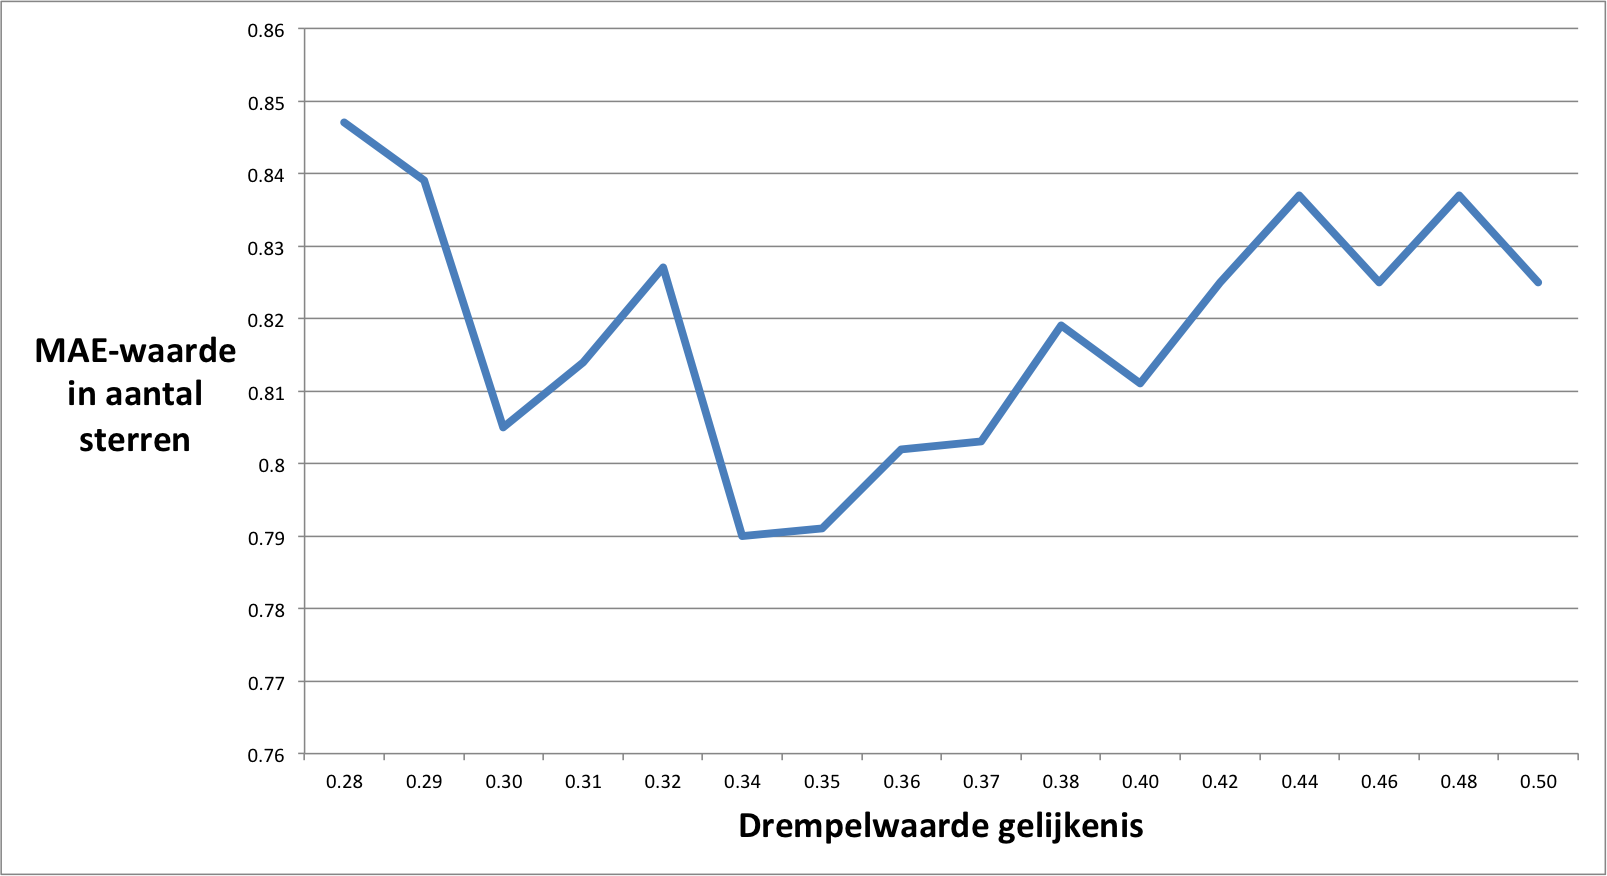
\includegraphics[scale=0.6]{fig/mae}       
\label{Figuur::mae} 
\end{center}
\begin{center} 
\centering 
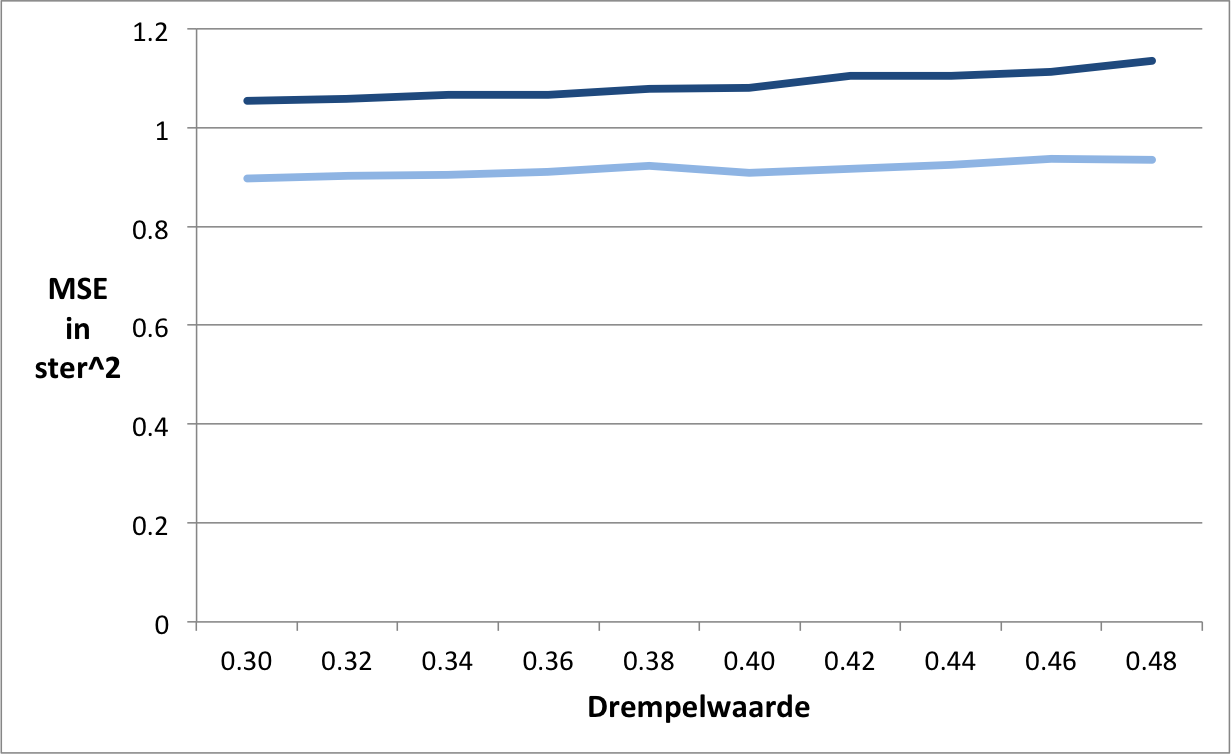
\includegraphics[scale=0.6]{fig/mse}  
    \label{Figuur::mse} 
\end{center}
\begin{center} 
\centering 
 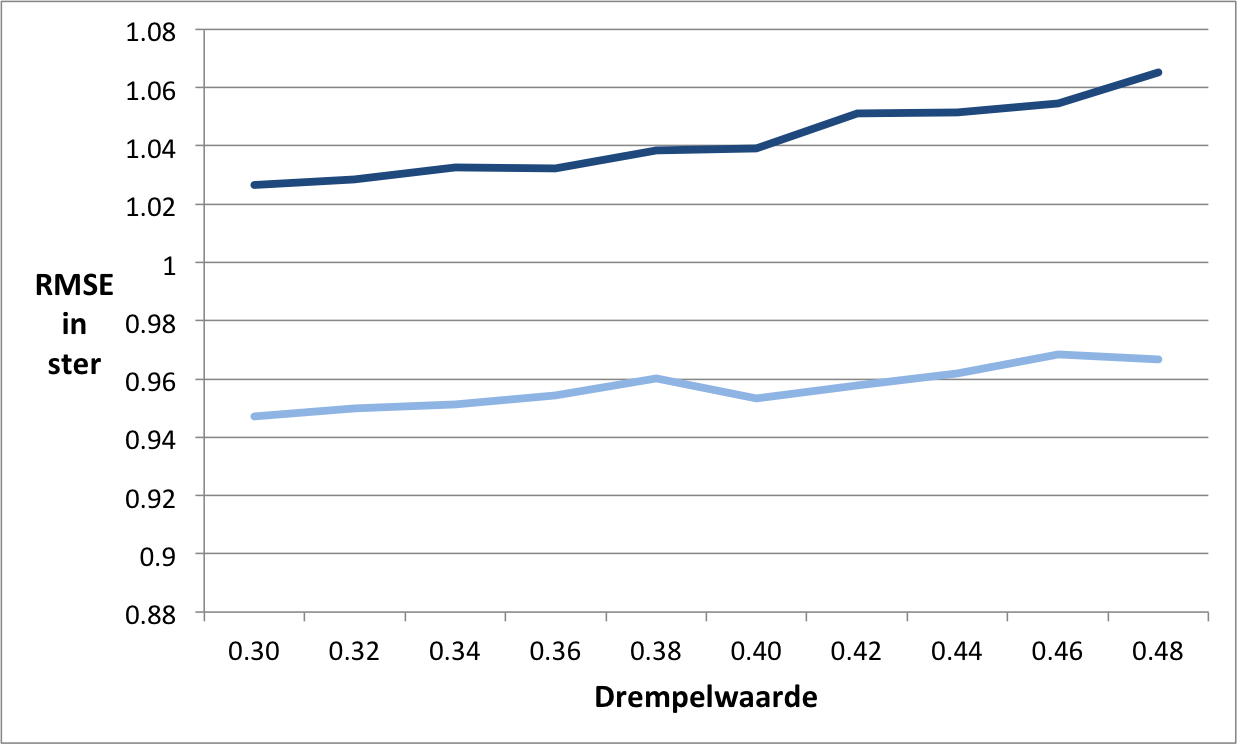
\includegraphics[scale=0.6]{fig/rmse} 
    \label{Figuur::rmse}  
\end{center}

\begin{center} 
\centering 
 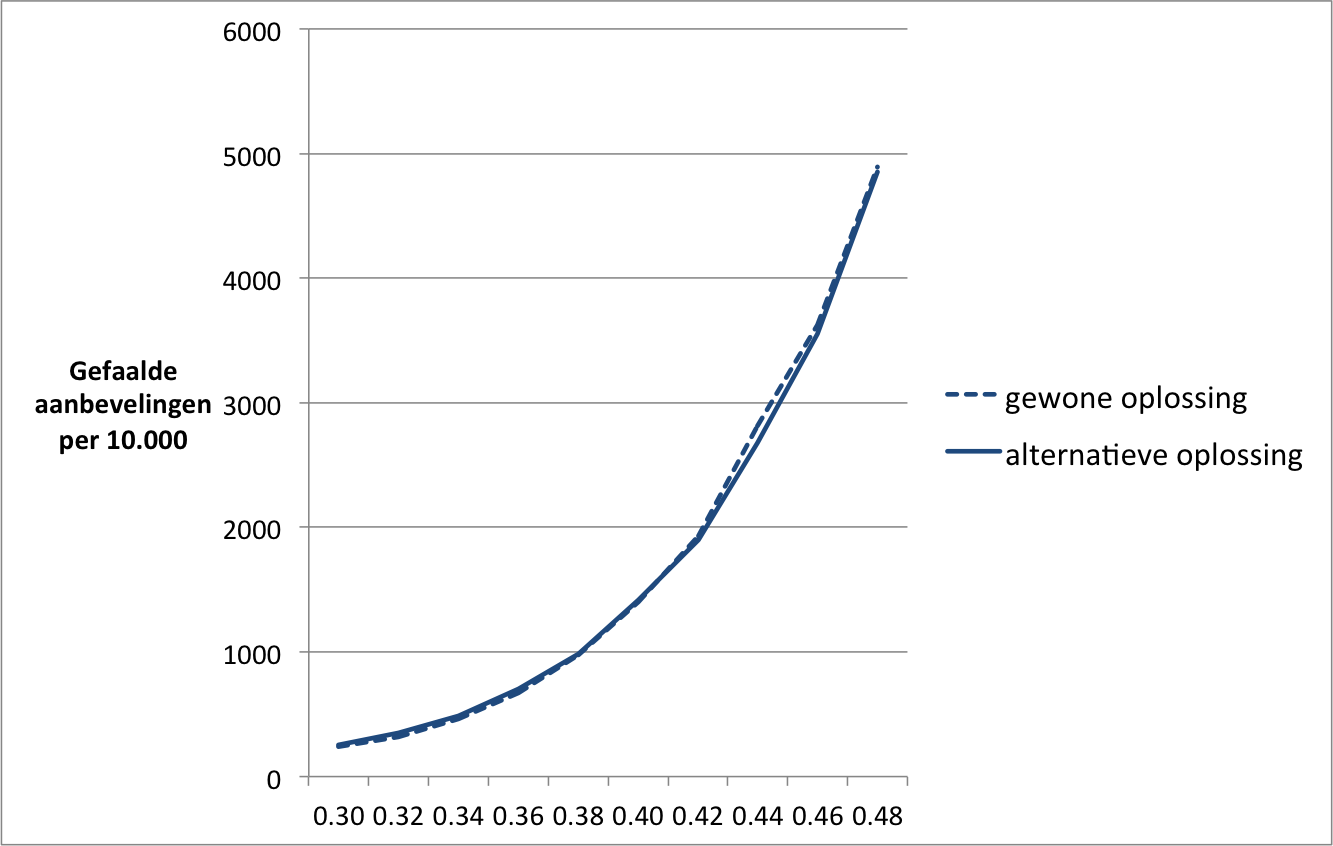
\includegraphics[scale=0.6]{fig/failed}  
    \label{Figuur::failed} 
\end{center}
Voor drempelwaarden groter dan 0.5 werden de aanbevelingen berekend op gemiddeld minder dan 10 beoordelingen van andere gebruikers. De MAE stijgt en er falen veel aanbevelingen, deze waarden zijn dus niet echt nuttig.
\begin{center} 
\centering 
 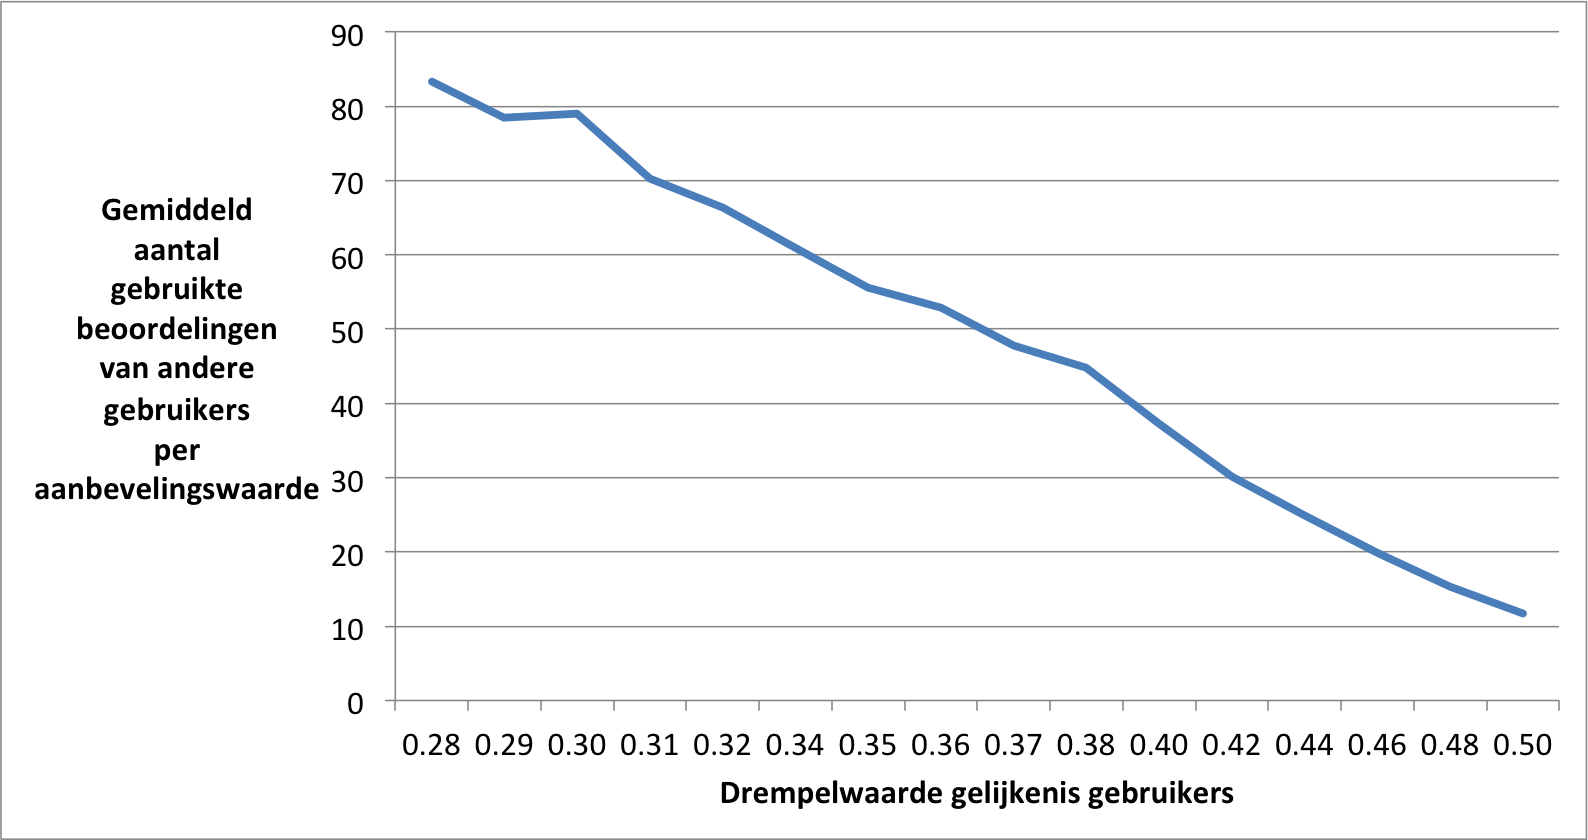
\includegraphics[scale=0.5]{fig/usedratings}     \label{Figuur::usedratings}  
\end{center}

Met een drempelwaarde in de buurt van 0.30 wordt de kleinste MAE, MSE en RMSEwaarden opgemeten in beide methodes. De alternatieve methode scoort duidelijk beter op nauwkeurigheid dan de werkwijze uit \cite{ZErkinDyn}. De MAE-waarde van de alternatieve methode komt in de buurt van 0.74, de oude wijze haalt maar een MAE van 0.82. Er wordt dus beter gescoord dan  de MAE-waarde 0.7964 van de privacyvriendelijke oplossing uit "Svd-based collaborative filtering with privacy\cite{Polat:2005:SCF:1066677.1066860}" besproken in \ref{randomisatie}. In dit artikel werd ook de MAE berekend voor een niet-privacyvriendelijke oplossing: 0.7146. Beide waarden werd berekend op identiek dezelfde dataset van MovieLens. Het verschil van de bekomen MAE 0.74 met de MAE van de niet-privacyvriendelijke methode 0.7146 is dus 0.0254 ster. Er wordt dus niet veel aan nauwkeurigheid ingeboet.
\section{Performantie}
\subsection{Het mobiele toestel}
Het mobiel \emph{device} moet het meeste werk leveren als de gebruiker zijn profiel uploadt. Dan encrypteert het toestel niet alleen de voorkeuren en de beoordelingen van de gebruiker, maar ook een nulwaarde voor de items die niet beoordeeld zijn. Dit gebeurt zodat de service provider niet weet welke items beoordeeld werden. Een andere optie is ook telkens een paar random items uit te kiezen en de nulwaarden hiervan mee te sturen. Het is hierbij wel mogelijk dat alle random items in een bepaalde groep liggen, waardoor de service provider toch smaken kan afleiden. Deze methode is dus $O(N+S)$ waarbij N staat voor het aantal items en S voor het aantal preferences.
In de praktijk komt dit overeen met 1,52 seconden op het testtablet \footnote{Samsung Galaxy Tab4 (7.0) Wi-Fi op Android 4.4.2} als er een richtwaarde genomen wordt van 30 preferences. 

\subsection{De aanbevelingsserver en de controleserver}
Server 1 en 2 moeten zware berekeningen verrichten en veel informatie over en weer sturen. Dit is vooral dankzij het multiplicatieprotocol en het drempelprotocol.  De performantie van het zwaarste protocol is $O(N(S+l^2))$ met l het aantal bits van een ge\"encrypteerde waarde. In de praktijk komt dit op onze server overeen met een tijd van 7 minuten 26 seconden bij 30 preferences. Achteraf gezien had de communicatie tussen de servers misschien beter op een lager niveau ge\"implementeerd geweest. Er zijn waarschijnlijk ook nog mogelijkheden om de oplossing te optimaliseren op dit gebied.
% appendices
\appendix

\bibliographystyle{plain}
\bibliography{refbib.bib}{}
% hier worden de appendices ingevoegd (\includes)

\backmatter

% eventueel: lijst van figuren en tabellen
%\listoffigures
%\listoftables

% lege pagina (!!)

% kaft

\end{document}
